\newif \ifdraft \drafttrue 
%\documentclass[10pt,twocolumn]{confpaper}
\documentclass[10pt,twocolumn,sigconf]{acmart}

\newif \ifappendix \appendixfalse

%\makeatletter \@input{texdirectives} \makeatother

%%%%%%%%%%%%%%%%%%%%  INCLUDES  %%%%%%%%%%%%%%%%%%%%%%%%%%
\usepackage{booktabs} % For formal tables

% Copyright
%\setcopyright{none}

%\setcopyright{acmlicensed}
%\setcopyright{rightsretained}
%\setcopyright{usgov}
%\setcopyright{usgovmixed}
%\setcopyright{cagov}
%\setcopyright{cagovmixed}


%Conference
\author{Vibhaalakshmi Sivaraman}
\affiliation{
	\institution{Princeton University}
}

\author{Srinivas Narayana}
\affiliation{
	\institution{MIT CSAIL}
}

\author{Ori Rottenstreich}
\affiliation{
	\institution{Princeton University}
}

\author{S. Muthukrishnan}
\affiliation{
	\institution{Rutgers University}
}

\author{Jennifer Rexford}
\affiliation{
	\institution{Princeton University}
}

% The default list of authors is too long for headers}
\renewcommand{\shortauthors}{V. Sivaraman et al.}

\copyrightyear{2017}
%\setcopyright{acmcopyright}
\acmConference[SOSR '17]{ACM Symposium on SDN Research}{April 3-4, 2017}{Santa Clara, CA} 
\acmISBN{978-1-4503-4947-5/17/04}
\acmPrice{\$15.00}
\acmDOI{http://dx.doi.org/10.1145/3050220.3050239}

\usepackage[normalem]{ulem}
\usepackage{amsmath, amssymb}
\usepackage{fullpage}
\usepackage{framed}
\usepackage{graphicx}
\usepackage{wrapfig}
%\usepackage{algorithm2e}
\usepackage[linesnumbered,ruled]{algorithm2e}
\usepackage{caption}
\usepackage{wrapfig}
\usepackage{subcaption}
\captionsetup{compatibility=false}
\usepackage{lipsum}
\usepackage[titletoc]{appendix}
\usepackage{hyperref} % http://ctan.org/pkg/hyperref
\hypersetup{%
  colorlinks = true,
  linkcolor  = black
}
\usepackage{csquotes}
\usepackage{xspace}
\usepackage{ragged2e}
\usepackage{fixltx2e}
\usepackage{amsmath,amsthm,amsfonts}
\usepackage{mdframed}
\usepackage{stmaryrd}
\usepackage{calc}
\usepackage[makeroom]{cancel}
\usepackage{algpseudocode}
%\usepackage{algorithm}
\ifappendix \usepackage[ruled,vlined]{algorithm2e} \fi
\usepackage{makecell}
\usepackage{lineno}
\def\linenumberfont{\footnotesize}
\usepackage{enumitem}
\usepackage[justification=justified, font=small]{caption}
\usepackage[export]{adjustbox}
\usepackage{bm}
\usepackage{amstext}
\usepackage{tabularx}
\usepackage{balance}
\usepackage{authblk}
\usepackage[export]{adjustbox}

\usepackage{listings}
\usepackage{color}

\lstset{
  columns=flexible,
  mathescape,
  keepspaces=true,
  escapeinside={(*}{*)},
  basicstyle=\ttfamily\small
}
 
\definecolor{codegreen}{rgb}{0,0.6,0}
\definecolor{codegray}{rgb}{0.5,0.5,0.5}
\definecolor{codepurple}{rgb}{0.58,0,0.82}
\definecolor{backcolour}{rgb}{0.95,0.95,0.92}

\graphicspath{ {figures/} }

\makeatletter
\renewcommand\AB@affilsepx{ , \protect\Affilfont}
\makeatother

%%%%%%%%%%%%%%%%%%%%  LOCALS  %%%%%%%%%%%%%%%%%%%%%%%%%%%%
\setlist[enumerate,1]{%
  label=\arabic*.,
}

\newlist{inlinelist}{enumerate*}{1}
\setlist*[inlinelist,1]{%
  label=(\roman*),
}

\newcommand{\system}{{\em NetASM}}
\newcommand{\lang}{SNAP\xspace}
\newcommand{\Lang}{SNAP\xspace}
\newcommand{\xFDD}{xFDD\xspace}
\newcommand{\xFDDs}{xFDDs\xspace}
\newcommand{\Tunnel}[1][footnotesize]{\code[#1]{DNS-tunnel-detect}\xspace}
\newcommand{\tsub}{\textsubscript}
\newcommand{\set}[1]{\{#1\}}
\newcommand{\sequence}[1]{<#1>}
\newcommand*{\Ucup}{\bigcup}
\newcommand{\fddl}{\sqsubset}
\newcommand{\atomic}{\mathsf{atomic}}
\newcommand{\snaptitle}[1]{\noindent {\bf #1}}

\newcommand{\eval}{\mathsf{eval}}
\newcommand{\evale}{\mathsf{eval}_e}
\renewcommand{\merge}{\mathsf{merge}}
\newcommand{\elog}{\mathsf{E}}
\newcommand{\Let}[3]{\text{let } {#1} ~=~ {#2} \text{in } {#3}}
\newcommand{\IfElse}[3]{\text{if } #1 \text{ then } #2 \text{ else } #3}
\newcommand{\ty}{\mathsf{ty}}
\renewcommand{\-}{\ensuremath{\vdash}}
\renewcommand{\=}{\ensuremath{\models}}
\newcommand{\uni}{\mathsf{unicast}}
\newcommand{\multi}{\mathsf{multicast}}
\newcommand{\LA}{anlys}
\newcommand{\PLA}{\LA\tsub{p}}
\newcommand{\Nodes}{\mathsf{Nodes}}
\newcommand{\Switches}{\mathsf{Switches}}
\newcommand{\Edge}{\mathsf{Edge}}
\newcommand{\StVar}{\mathsf{StateVars}}

\newcommand{\ignore}[1]{}
\newcommand{\TODO}[1]{\ifdraft {\color{red} \textbf{TODO:} {#1}} \fi }
\newcommand{\jrex}[1]{\ifdraft {\color{orange} \textbf{JR:} {#1}} \fi }

\newcommand{\ngs}[1]{{\color{red} \textbf{Srinivas:} {#1}}}
\newcommand{\vls}[1]{{\color{blue} \textbf{Vibhaa:} {#1}}}
\newcommand{\eg}{{\em e.g., }}
\newcommand{\etal}{{\em et al.}}
\newcommand{\vs}{{\em vs. }}
\newcommand{\ie}{{\em i.e., }}
\newcommand{\Sec}[1]{\S\ref{#1}}
\newcommand{\App}[1]{Appendix~\ref{#1}}
\newcommand{\TheSystem}{HashPipe\xspace}
\newcommand{\Baseline}{HashParallel\xspace}
\newcommand{\spacesaving}{space saving\xspace}
\newcommand{\SpaceSaving}{Space Saving\xspace}
\newcommand{\Spacesaving}{Space saving\xspace}
\newcommand{\NewPara}[1]{\noindent{\bf #1}}
\newcommand{\Alg}[1]{Algorithm~\ref{algo:#1}}
\newcommand{\Fig}[1]{Fig.~\ref{fig:#1}}

%%%%% THE location for new commands %%%%

\usepackage[hang,flushmargin]{footmisc} 
\usepackage{textcomp}
\newcommand{\cref}[1]{\textsection\ref{#1}}
%\usepackage{cleveref}
%\crefname{section}{\S}{\S\S}
%\Crefname{section}{\S}{\S\S}

\newsavebox\CBox
\newcommand\hcancel[2][0.5pt]{%
	\ifmmode\sbox\CBox{$#2$}\else\sbox\CBox{#2}\fi%
	\makebox[0pt][l]{\usebox\CBox}%  
	\rule[0.5\ht\CBox-#1/2]{\wd\CBox}{#1}}
%%%%%%%%%%%%%%%%%%%%  LANGUAGE COMMANDS  %%%%%%%%%%%%%%%%%%%%%%%%%%%%

\newcommand{\code}[2][footnotesize]{\begin{#1}\texttt{#2}\end{#1}}
\newcommand{\match}[2]{#1 = #2}
\newcommand{\modify}[2]{#1 <- #2}

\newcommand{\union}[2]{#1+#2}
\newcommand{\seq}[2]{#1;#2}
\newcommand{\inters}[2]{#1 \& #2}
\newcommand{\id}{id}
\newcommand{\drop}{drop}
\newcommand{\pstar}[1]{#1\textsuperscript{*}}
\newcommand{\ifelse}[3]{if #1 then #2 else #3}
\newcommand{\boldifelse}[3]{\textbf{if} #1 \textbf{then} #2 \textbf{else} #3}
\newcommand{\negate}[1]{$\sim$#1}
\newcommand{\pp}{\text{\code{++}}}
\newcommand{\mm}{\text{\code{-{}-}}}

\newcommand{\Expr}{\mathsf{Expr}}
\newcommand{\Pol}{\mathsf{Pol}}
\newcommand{\Pred}{\mathsf{Pred}}
\newcommand{\Packet}{\mathsf{Packet}}
\newcommand{\Log}{\mathsf{Log}}
\newcommand{\St}{\mathsf{St}}
\newcommand{\Store}{\mathsf{Store}}
\newcommand{\Val}{\mathsf{Val}}
\newcommand{\consistent}{\mathsf{consistent}}
\newcommand{\harpoon}{\overset{\rightharpoonup}}

\newcommand{\stgraph}{\textproc{st-dep}}
\newcommand{\R}{\textproc{r}}
\newcommand{\W}{\textproc{w}}
%%%%%%%%%%%%%%%%%%%%  HIGHLIGHTING % %%%%%%%%%%%%%%%%%%%%%

\newcommand{\highlighttext}[2][yellow]{{\setlength{\fboxsep}{0pt}\colorbox{#1}{#2}}}

\newcommand{\highlight}[2][yellow]{\mathchoice%
  {{\setlength{\fboxsep}{0pt}\colorbox{#1}{$\displaystyle#2$}}}%
  {{\setlength{\fboxsep}{0pt}\colorbox{#1}{$\textstyle#2$}}}%
  {{\setlength{\fboxsep}{0pt}\colorbox{#1}{$\scriptstyle#2$}}}%
  {{\setlength{\fboxsep}{0pt}\colorbox{#1}{$\scriptscriptstyle#2$}}}}

%%%%%%%%%%%%%%%%%%%%%  SPACING % %%%%%%%%%%%%%%%%%%%%%%%
\setlength{\abovecaptionskip}{0.5mm}
\setlength{\belowcaptionskip}{-2mm}
%%%%%%%%%%%%%%%%%%%%  TITLE/AUTHORS  %%%%%%%%%%%%%%%%%%%%%

%\date{}
%\title{\ttlfnt{Smoking Out the Heavy-Hitter Flows with HashPipe}}

%\author{
%Paper \# \ "paper num",  
%\pageref{lastpage} pages
%\aufnt{\AUTHORS} \\
%\affaddr{Affiliation}
%}


%%%%%%%%%%%%%%%%%%%%  START OF DOCUMENT  %%%%%%%%%%%%%%%%%
\begin{document}
%%\title{Smoking Out the Heavy-Hitter Flows with HashPipe}
\title{Heavy-Hitter Detection Entirely in the Data Plane}
\thispagestyle{empty}

%\author{Ben Trovato}
%\authornote{Dr.~Trovato insisted his name be first.}
%\orcid{1234-5678-9012}
%\affiliation{%
%  \institution{Institute for Clarity in Documentation}
%  \streetaddress{P.O. Box 1212}
%  \city{Dublin} 
%  \state{Ohio} 
%  \postcode{43017-6221}
%}



%\email{trovato@corporation.com}
%\author[1]{Vibhaalakshmi Sivaraman}
%\author[2]{Srinivas Narayana}
%\author[1]{Ori Rottenstreich}
%\author[3]{\\S. Muthukrishnan}
%\author[1]{Jennifer Rexford}
%\affil[1]{Princeton University}
%\affil[2]{MIT CSAIL}
%\affil[3]{Rutgers University}
%\setcounter{Maxaffil}{0}
%\renewcommand\Affilfont{\small}

\begin{abstract}

% doing this entirely in the dataplane
Identifying the ``heavy hitter'' flows or flows with large traffic volumes in the dataplane is important for several applications \emph{e.g.,} flow-size aware routing, DoS detection and traffic engineering.
%Understanding which  traffic flows consume the most bandwidth is useful for load
%balancing, detecting DoS attacks, and traffic engineering. Identifying these
%``heavy hitter'' flows in the data plane enables applications that distinguish
%between packets belonging to heavy and light flows at packet-processing time,
%\emph{e.g.,}
%to route heavy flows or DoS traffic differently. 
However, measurement in the data plane is constrained by the need for line-rate processing (at 10-100Gb/s) and
limited memory in switching hardware. We propose HashPipe, a heavy hitter detection algorithm using emerging programmable data planes.
HashPipe implements a pipeline of hash tables which retain counters for heavy flows in various stages while evicting lighter flows over time.
We prototype HashPipe in P4 and
evaluate it with CAIDA packet traces from an ISP backbone link. We find that
HashPipe identifies 95\% of the 300 heaviest flows with less than 80KB of memory on a trace that contains 500,000 flows.
\end{abstract}


% \begin{CCSXML}e
% <ccs2012>
% <concept>
% <concept_id>10003033.10003068</concept_id>
% <concept_desc>Networks~Network algorithms</concept_desc>
% <concept_significance>500</concept_significance>
% </concept>
% <concept>
% <concept_id>10003033.10003099.10003105</concept_id>
% <concept_desc>Networks~Network monitoring</concept_desc>
% <concept_significance>500</concept_significance>
% </concept>
% <concept>
% <concept_id>10003033.10003099.10003102</concept_id>
% <concept_desc>Networks~Programmable networks</concept_desc>
% <concept_significance>300</concept_significance>
% </concept>
% </ccs2012>
% \end{CCSXML}

%ccsdesc[500]{Networks~Network algorithms}
%ccsdesc[500]{Networks~Network monitoring}
%ccsdesc[300]{Networks~Programmable networks}


\keywords{Software-Defined Networks; Network Monitoring; Programmable Networks; Network Algorithms} %e filled

\maketitle


%\AcmCopyright
%\ToAppear
%\begin{sloppypar}

%\ifthenelse{\equal{\onlyAbstract}{no}}{% !onlyAbstract


\section{Introduction}
\label{sec:intro}

%Accurate measurement of network traffic is important for management tasks,
%%  such as traffic engineering, provisioning capacity, and diagnosing and
%% stopping DoS attacks.
%as lack of visibility into the network can lead to poor performance and costly
%outages.
%% Further, as packet-processing becomes increasingly flexible
%% \cite{mckeown2008openflow, bosshart2014p4, domino}, it is important to drive
%% fine-grained network control through accurate monitoring data. 
%As a result, both industry and academia have actively invested in improving the
%state of the art~\cite{cisco-netflow, estan2002new, int, yu2013software,
 % li2016flowradar, univmon}.

Many network management applications can benefit from finding the set of flows
contributing significant amounts of traffic to a link: for example, to relieve
link congestion~\cite{netscope}, to plan network
capacity~\cite{att-deriving-traffic-demands}, to detect network anomalies and
attacks~\cite{network-wide-anomalies}, or to cache forwarding table
entries~\cite{cacheflow}.
%
Further, identifying such ``heavy hitters'' at small time scales (comparable to
traffic variations~\cite{hedera, microTE}) can enable dynamic routing of heavy
flows~\cite{devoflow, planck} and dynamic flow scheduling~\cite{pifo}.

It is desirable to run heavy-hitter monitoring at all switches in the network
all the time, to respond quickly to short-term traffic variations. {\em Can
  packets belonging to heavy flows be identified as the packets are processed in
  the switch}, so that switches may treat them specially?

Existing approaches to monitoring heavy items make it hard to achieve
reasonable accuracy at acceptable overheads (\Sec{sec:related}). While packet
{\em sampling} in the form of NetFlow~\cite{cisco-netflow} is widely deployed,
the CPU and bandwidth overheads of processing sampled packets in software make
it infeasible to sample at sufficiently high rates (sampling just 1 in 1000
packets is common in practice~\cite{sflow-sampling-rate}). An alternative
is to use sketches, \eg \cite{cormode2005improved, li2016flowradar,
  yu2013software, univmon} that {\em hash} and {\em count} all packets in switch
hardware. However, these systems incur a large memory overhead to retrieve the heavy hitters
%required to estimate counts for {\em all} flows-
--- ideally, we wish to use memory proportional to the number of the heavy flows (say the top hundred). There may be tens of thousands of
active flows any minute on an ISP backbone link (\Sec{sec:evaluation}) or a data
center top-of-rack switch \cite{theo-dc-traffic}.

Emerging programmable switches~\cite{RMT,barefoot-tofino,cavium-xpliant} allow
us to do more than sample, hash, and count, which suggests opportunities to run
novel algorithms on switch hardware. While running at line rates of
10-100 Gbps per port over 10-100 ports, these switches can be programmed to keep and
manipulate state over multiple packets, \eg to keep flow identifiers as keys
along with counts, or perform comparisons between a packet's flow count and the
count stored in the state. Stateful manipulations can also be {\em pipelined}
over multiple stages, with the results carried by the packet from one stage to
the next.

However, switches are also constrained by the need to maintain high
packet-processing throughput, having:
\begin{itemize}
\item a deterministic, small time budget (1 ns \cite{RMT}) to manipulate state
  and process packets at each stage;
\item a limited number of accesses to memory storing state at each stage (typically just one read-modify-write);
\item a limited amount of memory available per stage (\eg 1.4MB shared across forwarding and monitoring~\cite{RMT}); 
%\item a limited amount of computation and boolean operations that are doable at each stage; and
\item a need to move most packets just once through the pipeline, to
  avoid stalls and reduced throughput
  (``feed-forward''~\cite{minions}).
\end{itemize}
%% accesses to the state per stage (typically just one), limited per-stage fast
%% memory (\eg 1.4MB~\cite{bosshart2014p4} SRAM shared across everything on the
%% switch), and a ``feed-forward'' model of processing where packets cannot return
%% to a previous stage in the pipeline without costly ``recirculation" of the
%% traffic.

%% % what the problem is and Why network operators want to know information, do people really need this?
%% Network measurements are crucial to effective network management. These measurements play a critical role in traffic engineering, understanding network vulnerabilities, preventing DDoS attacks, scalable threshold accounting, and scalable queue management \cite{estan2002new}. Particularly, identifying the flows that make the largest contribution to traffic across a particular link helps us reason about where congestion may be arising from, denial-of-service attacks and high-level trends in the traffic patterns. Knowing the heavy hitters is useful not only for reporting to the network operator, but also for acting on heavy hitters directly in the data plane, for example, to load balance traffic such that heavy hitters (elephants) are sent on disjoint paths. Ideally, network operators want to be able to gather these measurements from all points in a network, throughout the period when a network is on % rephrase this
%% and without imposing any overheads or slowing down the per-packet processing speed.

%% % Next generation of switching chips that can do these things
%% In the meantime, there has been significant development in the hardware realm. The next generation of reconfigurable switch hardware \cite{bosshart2014p4} enables programmers/operators to specify customizable and useful state that is tracked directly in the data path of the packets on the switch. In fact, such data plane programs can manipulate this state in complex ways — both to choose which state is kept (which could be useful in deciding which flows to retain state for) and how that state is updated (helps decide between increment counters, merging multiple counters or resetting them). The fact that you could read such state directly in the data path also means you could choose to process packets in different ways based on the state: e.g., route heavy flows across different paths than short-lived flows. State can also be carried through the multiple stages in the packet processing pipeline within switches as metadata which could be used to differentiate between packets on a stage to stage basis. These switches are easily reconfigurable as opposed to custom-designed hardware. And all of this happens at the line rate supported by the switch, e.g., 64 ports of 10-100Gb/s!

%% % downsides
%% %there is exactly one location that we can read
%% % it is not possible to read more than one in one stage, but you can make that up by pipelining the table and getting multiple reads across multiple stages
%% % all ways are hands are tied behind back - do things in a pipelined fashion
%% While these new switches offer a lot of programmability, they do come with a lot of constraints in order for programs to be feasible at line-rate. The amount of memory available on the chip is limited. This means that one cannot maintain data per TCP connection in a typical network \cite{li2016flowradar}. Further, state is local to each pipelined stage and the pipelined stages follow a {\em{feed-forward model}} {\em{i.e.}} a given packet cannot be sent back to an earlier stage in the pipeline since the pipelining enables the processing of multiple concurrent packets, one in each stage. Together, these two constraints imply that all modifications to the state associated with a particular stage need to be completed before the packet moves on to the next stage. Further, deterministic time operations are needed to maintain switch line-rate which makes ideas like scanning the entire register challenging. This also means that maintaining complex yet space-efficient data structures like a heap aren't feasible at line rate since the operations needed to keep them compact and sorted involve multiple reads and writes. 
%% %Further, if there is a write back operation in the stage, that write back is dependent on exactly one read at the same location - essentially one atomic read, modify, operation - writing back to one location based on multiple reads might involve considerably longer clock cycles

%% % time scale issues - sampling doesn't catch everything (netflow samples about 1 in thousand), how frequently you get information and how would you aggregate it
%% % is link speed getting higher - would this imply that you have to sample at a lower rate - what should be the sampling rate if you want to report things at a certain rate because of the current link speed - NETFLOW is run on only certain switches, but we could do this on every switch - Overhead, accuracy and time of reporting - OpenSketch may have some point here
%% %how is it done today - sampling, collecting info, netflow, etc
%% %There is all this theory discussion, but most of them aren't used in practice
%% %HH: both top K and thresholded: important --> obvious.
%% The particular problem of heavy hitter detection, both in terms of identifying all flows with a size above a threshold or identify the Top-K flows by size, has been extensively researched (\cite{estan2002new}, \cite{schweller2004reversible}, \cite{cormode2005improved}, \cite{metwally2005efficient}, \cite{jose2011online}). However, we require schemes that ideally keep  a small amount of state, update that state in deterministic (constant) time, use a small number of memory accesses per packet, a small number of pipeline packet processing stages per packet and can read off accurate counts for each traffic aggregate in the data plane itself, to support “online” decisions for packets from heavy flows. And we require that all this be feasible with emerging programmable switch hardware \cite{RMT}. A majority of the algorithms (\cite{manku2002approximate}, \cite{misra1982finding}, \cite{li2016flowradar}) aren’t useful in practice because they do not satisfy one of these requirements.

%% % table of related work You could even itemize the points, or make a small table showing how the existing schemes falter in one or more of these requirements.
%% The few algorithms that can be implemented \ignore{\cite{estan2002new}, \cite{netflow}} are either based on sampling or  sketching techniques. While sampling-based approaches become less accurate as increasing link speeds \ignore{cite} force smaller sampling rates leading to higher chances of missing out on important flows, majority of sketching techniques (\cite{cormode2005improved}, \cite{li2016flowradar}, \cite{charikar2002finding}, \cite{cormode2005s}) are meant to maintain information for all flows and are hence not optimized to accurately report the heavy hitters alone. However, given the capabilities of newer and more programmable hardware, could we closely model one of the more space-efficient algorithm at line-rate without trading off much accuracy?

% why is space-saving the right algorithm to go off from 
% is there a case for controller overhead reduction? 
% simplicity: (1) controller overhead reduction (2) low "complexity" in the data
% plane (3) amount of information sent to the controller
We present \TheSystem,  an algorithm to track the $k$ heaviest flows with high
accuracy and $O(k)$ space (\Sec{sec:algorithm}) using the features and constraints of programmable switches. \TheSystem maintains both the
flow identifiers (``keys'') and counts of heavy flows in the switch, in a
pipeline of hash tables. 
%Packets flow from one stage to next and at each stage, the ``state'' carried by the packet maybe modified by the counts in that hash stage. This is distinct for example from generic multistage algorithms where the information passed between stages is contained in the program variables, whereas here the information flow is via the packets.  
%We design a new heavy hitter detection algorithm using \TheSystem as follows. 
When a packet hashes to a location in the first stage of the pipeline,
its counter is updated (or newly inserted) if there is a {\em hit} (or an empty
slot). If there is a {\em miss}, the new key is inserted at the expense of the
existing key. In all downstream stages, the key and count of the just evicted item are carried along with the packet. The key just evicted is looked up in the current stage's hash table. Between the key looked up in the hash table and the one carried, the key with the {\em larger count} is retained in the hash
table, while the other is carried along with the packet---either to the next
stage, or totally removed from the switch if the packet is in its last
stage. Hence, \TheSystem ``smokes out'' the heavy keys within the limited
available memory, using pipelined operation to sample multiple locations in the
hash tables, and evicting lighter keys that occupy memory in favor of heavier
keys with updates to exactly one location per stage. %% Our algorithm is inspired by
%% the strategy used by the {\em space-savings} algorithm
%% \cite{metwally2005efficient}.\jrex{mention of the space-savings algorithm
%% arises abruptly, leaving the reader wondering how similar it is.  maybe we
%% could mention it earlier as a transition from the point that we need to keep
%% space proportional to k.}

We prototyped \TheSystem  in P4~\cite{bosshart2014p4} (\Sec{sec:prototype}) and
tested it on the public-domain behavioral switch model \cite{p4-bm}. %% We also
%% provide some basic analytical bounds for the estimation errors of our algorithm
%% (\Sec{sec:analysis}). 
We evaluate \TheSystem with a packet trace containing over 500 million packets
from an ISP backbone link, and show that \TheSystem can provide high accuracy
(\Sec{sec:evaluation})---less than 5\% false negatives and 0.001\% false
positives when reporting 300 heavy hitters (keyed by transport five-tuple) with
just 4500 counters (less than 80KB) overall, while the trace itself contains 500,000 flows. At 80KB, \TheSystem also outperforms sample and hold (by over $15\%$) as well as an augmented version of count-min sketch (by $3$-$4\%$).  We
also show that the errors in identification and count estimation are much lower
on the larger flows among the top $k$.

%% \begin{itemize}
%% \item An algorithm, \TheSystem, that maintains the top $K$ heavy items on switches
%%   accurately with O($K$) counters;
%% \item A prototype implementation of \TheSystem in P4;
%% \item An analysis of the \TheSystem algorithm that bounds the over- and
%%   under-estimation errors on average; and
%% \item An evaluation with traces from an ISP backbone, which shows a false
%%   positive and negative error rates of XXX.
%% \end{itemize}

%% In order to convert the space-saving algorithm
%% into a version feasible on commodity hardware, we approximate the minimum by
%% sampling a constant number of locations in the table and not the entire
%% table. Further, we compute the minimum in a feed-forward manner by spreading
%% state across multiple stages of the match-action table. This minimizes the
%% number of reads per location as well as eliminates the need for packet
%% re-circulation. Though making Space-Saving hardware amenable has some visible
%% tradeoffs, using a memory of just xxx bytes, we could track all TCP connections
%% heavier than a fraction xxx of overall traffic in the network with a xx\% false
%% positive rate and xx\% false negative rate. The tracked flows had a xx\% average
%% error in the counters. We also prototyped the algorithm in P4
%% \cite{bosshart2014p4}. % and compile it to a target.


% Main contribution: new algorithm that is implementable on hardware - sweet spot given the capabilities of emerging switch hardware

%Section 2 could be just the related work





\section{Background on Heavy-Hitter Detection}
\subsection{Problem Formulation}
\label{sec:problem}

\NewPara{Heavy hitters.} ``Heavy hitters'' can refer to all flows that are
larger (in number of packets or bytes) than a fraction $t$ of the total packets
seen on the link (the ``threshold-$t$'' problem). Alternatively, the heavy
hitters can be the top $k$ flows by size (the ``top-$k$''
problem). Through the rest of this paper, we use the ``top-$k$'' definition. %The two problems are nearly interchangeable, where a reasonable
%threshold $t$ can be used to identify the $k$ largest flows, and vice versa.

\NewPara{Flow granularity.} Flows can be defined at various levels of
granularity, such as IP address (\ie host), transport port
number (i.e., application), or five-tuple (\ie transport connection). With a
finer-grained notion of flows, the size and number of keys grows, requiring more
bits to represent the key and more entries in the data structure to track 
the heavy flows accurately.

\NewPara{Accuracy.} A technique for detecting heavy hitters may have false
positives (\ie reporting a non-heavy flow as heavy), false negatives (\ie not
reporting a heavy flow), or an error in estimating the sizes of heavy flows.
The impact of errors depends on the application.  For example, if the switch
performs load balancing in the data plane, a few false negatives may be
acceptable, especially if those heavy flows can be detected in the next time
interval.  As another example, if the network treats heavy flows as suspected
denial-of-service attacks, false positives could lead to unnecessary alarms that
overwhelm network operators. When comparing approaches in our evaluations, we
consider all three metrics.
%% and penalize approaches with a very high rate of either false positives or
%% false negatives.

\NewPara{Overhead.} The overhead on the switch includes the total amount of
memory for the data structure, the number of matching stages used in the switch
pipeline (constrained by a switch-specific maximum, say 16~\cite{RMT}). The
algorithms are constrained by the nature and amount of memory access and
computation per match stage (\eg computing hash functions). On high-speed links,
the number of active five-tuple flows per minute can easily be in the tens of
thousands, if not more. Our central goal is to maintain data-plane state that is proportional to the target number $k$ of heavy hitters (\eg $5k$ or
$10k$), rather than the number of active flows. In addition, we would like
to use as few pipeline stages as possible, since the switch also needs to
support other functionality related to packet forwarding and access control.

%Given a single switch $s$, and a total of $n$ active flows as observed at this switch within a given time interval $[t_k, t_{k+1}]$, we wish to identify the heavy hitters. This could refer to all those flows which are larger than a threshold size or the top $k$ flows, by size, for a given $k$. For convenience sake, lets refer to the former as "heavy hitters by threshold" and the larger as "top-k". By \textbf{size} of a particular flow, we refer to the number of packets belonging to that flow that are observed at this switch $s$. The threshold is a certain (predetermined) fraction of the total number of packets across all the active flows. This threshold could also be translated into an appropriate $k$ value is if the problem is phrased as reporting the top $k$ flows at this switch, if one has some knowledge of what the relative distribution of the flow sizes are.  

%In essence, given the input $n$ flows (each identified by a unique identifier) that between them refer to all the packets arriving at the switch $s$ during the time interval$[t_k, t_{k+1}]$, we are interested in the set $A$ where $A$ represents either the heavy hitters by threshold or the top k.
% should we just use one of them?

%\begin{framed}
%\textbf{Input:} Set $F = \{f_1, f_2, \dots, f_n\}$ and a threshold $\phi$ or a number $k$ \\
%\textbf{Output (Heavy hitters by threshold):} Set $A$ s.t. $A \subset F$ and
%$$ for \  all \  a \in A, \  Size(a) \geq \displaystyle \phi \sum_{f \in F} Size(f) $$
%textbf{Output (Top-K):} Set $A$ s.t. $A \subset F$ and $\vert A \vert = k$ and $$ for \  all \  a \in A, \  Size(a) \geq \displaystyle Size(f) \ for \  all \ f \in F - A  $$
%\end{framed}

%In the context of this problem, flows can be defined at different levels of granularity. They could group packets based on just the source or destination ip address, or based on port if one is interested in the applications producing most traffic or by the 5-tuple. Regardless, of how granular the flow is defined, the number of active flows is typically extremely large (of the order of "blank") %fill
%and maintaining per-flow data is not scalable given the constraints of the hardware. This means that any proposed approach can maintain information for only a subset of all the flows. Yet, the number and complexity of the operations should be feasible at line-rate in the dataplane without significant overheads. In addition, the amount and frequency of information sent to the controller should also be reasonable % expand this further, give numbers.%
%and majority of this information should be available right in the dataplane for applications that might want to use it without going through the controller. Further, our goal is for the algorithm to be implementable on commodity switches without needing custom hardware optimized for the purposes of this particular measurement problem. This involves ensuring that packets are only fed forward, traverse each table stages once without recirculation or stalling and perform a constant number of reads/writes in each stage.

%Our goal in terms of accuracy for the approach and what we might consider good enough is highly dependent on the application that is using the information on the heavy hitters. For example, if we want to perform load balancing in the dataplane, missing a few heavy hitters might not be too bad especially if we re-randomize the hash functions in the next interval and they continue to be heavy hitters in the next interval. However, in this context, if we report a large number of false positives at the cost of not missing any true heavy hitters, it could cause an explosion of state to maintain load balancing information for the large number of flows that aren't actually heavy hitters. Similarly, if the goal is fraud and/or anomaly detection, a few false positives or negatives might not be too bad if we could get more information in the next time interval and correlate it with the current information to make it more accurate. However, a large number of either could be terrible either in terms of missing anomalies or causing significant overhead and unnecessarily flagging "rightful" flows. Hence, when comparing approaches, we prefer those with a very small percentage of false positives or negatives, but penalize approaches with an extremely high rate of either even if it is at the cost of the other metric being 100\%.

%\subsection{Hardware Model} - already in the intro
% explain the 


%The internal hardware within every switch that is exploited to perform any classification or counting based on packet fields is the \textbf{content addressable memory (CAM)} or high-speed memory within match-action tables. A match-action table determines what action should be executed when a packet matches a certain criteria.The CAM within each of these tables stores a tag or a field to search on and an associated value for each tag. This value can be a rule that specifies what action needs to be taken for a particular class in the case of a "match-action rule table" or could be a counter that needs to be incremented to track the packets belonging to that class. The existing values in the CAM are compared parallely until an exact match is found and it is this parallel comparison process that makes the CAM fast and ideal for high-speed packet processing. There could be a single match-action table or a series of tables one after the other within a particular switch that process a packet. .

%With the advent of languages like P4 \cite{bosshart2014p4}, it has become easier to program how switches in the network process packets. The language provides an easier interface with lower level rules like OpenFlow \cite{mckeown2008openflow} that directly communicate with the network infrastructure and helps program the dataplane. It has also made it possible to make changes to these rules while packets are in transit and based on these packets themselves as opposed to going through the controller. The language is protocol independent and hence, is able to interface with a wide range of final targets/hardware making it easier to program all of them. In particular, the language lets you define individual table stages, the actions within them, the match rules for those actions and also supports read-modify-write operations for these rules/fields while the packet is in transit. These features are critical to building a key-value store with dynamic updates as the packet traverses the network that enables us to track flow information. Along with the language framework, there is also a reference swtich provided on which any of the programs created through this interface can be run.

% \subsection{Related Work}


\subsection{Existing Solutions}\label{sec:related}

The problem of finding heavy flows in a network is an instance of the ``frequent
items'' problem, which is extremely well studied in the streaming algorithms
literature~\cite{hh-cormode-survey}.
%
While high accuracy and low overhead are essential to any heavy hitter detection
approach, we are also specifically interested in implementing these algorithms
within the constraints of emerging programmable switches
(\Sec{sec:intro}).
%
We classify the approaches into two broad categories, {\em sampling} and {\em
  streaming,} discussed below.
%% \jrex{I think it'd be better to start with sketches like count-min sketch that
%%   make no effort to thin out or evict small flows, so you can transition from
%%   that to schemes that do such as count-min-with-cache, sample-and-hold, and
%%   finally space-savings.}

\NewPara{Packet sampling} using NetFlow~\cite{cisco-netflow} and sFlow~\cite{sflow}
is commonly implemented in routers today. These technologies record a subset of
network packets by sampling, and send the sampled records to collectors for
analysis. To keep packet processing overheads and data collection bandwidth low,
NetFlow configurations in practice use aggressively low sampling probabilities,
\eg 1\% or even 0.01\% \cite{sflow-sampling-rate, netflow-sampling-rate}. Such
undersampling can impact the estimation accuracy.

Sample and hold \cite{estan2002new} enhances the accuracy of packet sampling by
keeping counters for {\em all} packets of a flow in a ``flow table,'' once a
packet from that flow is sampled. However, implementing the flow table is
challenging, since the flow table requires a memory that is %sufficiently fast (to be read/written to by each packet) 
sufficiently large (to hold the necessary flow
entries).

Designing a large flow table\footnote{Large exact-match lookups are typically
  built with SRAM, as large TCAMs are expensive.} for fast packet {\em lookup}
is well-understood: hash table implementations are already common in switches,
for example in router FIBs and NetFlow~\cite{li2016flowradar}.
%
However, it is challenging to handle hash collisions when {\em adding} flows to
the flow table, when a packet from a new flow is sampled.
%
Some custom hardware solutions combine the hash table with a ``stash'' that
contains the overflow, \ie colliding entries, from the hash
table~\cite{sram-tcam-learning}. But this introduces complexity in the switch
pipeline, and typically involves the control plane to add entries into
the stash memory.
%
Ignoring such complexities, we evaluate sample and hold in \Sec{sec:evaluation}
by liberally allowing the flow table to lookup packets {\em anywhere} in a {\em
  list} that can grow up to a pre-allocated size.

\NewPara{Streaming algorithms} implement data structures with bounded memory size
and processing time per packet, while processing {\em every packet} in a large
stream of packets in one pass. The algorithms are designed with provable
accuracy-memory tradeoffs for specific statistics of interest over the
packets. While these features make the algorithms attractive for network
monitoring, the specific algorithmic operations on each packet determine
feasibility on switch hardware.

Sketching algorithms like count-min sketch~\cite{cormode2005improved} and count
sketch~\cite{charikar2002finding} use per-packet operations such as hashing on
packet headers, incrementing counters at hashed locations, and determining the
minimum or median among a small number of the counters that were hashed
to. These operations can all be efficiently implemented on switch
hardware~\cite{yu2013software}.
%
However, these algorithms do not track the flow identifiers of packets, and hash
collisions make it challenging to ``invert'' the sketch into the constituent
flows and counters.
%
Techniques like group testing~\cite{group-testing}, reversible sketches
\cite{schweller2004reversible}, and FlowRadar~\cite{li2016flowradar} can decode
keys from hash-based sketches. 
%
However, it is challenging to read off an accurate counter value for a packet in
the switch pipeline itself since the decoding happens off the fast packet-processing
path.
%
%Further, all the above approaches use the available memory to estimate {\em all}
%flows---not just the heavy ones.
%%(i) take up too many counter updates per packet
%%(ii) use too many counters overall too! accuracy-memory tradeoff not great

Counter-based algorithms~\cite{misra1982finding,manku2002approximate} focus on measuring the heavy
items, maintaining a table of flows and corresponding counts. They employ
per-counter increment and subtraction operations, but potentially all counters
in the table are updated during some flow insertions.
Updating multiple counters in a single stage is challenging within the deterministic time budget for each packet.
%Such worst-case table updates are not possible within the deterministic time budget for each packet.

Space saving~\cite{metwally2005efficient} is a counter-based algorithm
that only uses $O(k)$ counters to track $k$ heavy flows, achieving the best
memory usage possible for a deterministic heavy-hitter algorithm. Space saving
only updates one counter per packet, but requires finding the item with the
minimum counter value in the table. Unfortunately, scanning the entire table on
each packet, or finding the minimum in a table efficiently, is not directly
supported on emerging programmable hardware (\Sec{sec:intro}). Further,
maintaining data structures like sorted linked
lists~\cite{metwally2005efficient} or priority queues~\cite{pifo} requires
multiple memory accesses within the per-packet time budget. %% Recently proposed
%% advances in switch hardware may make such data structures
%% possible~\cite{pifo}.
%
However, as we show in \Sec{sec:algorithm}, we are able to adapt the key ideas of the space saving algorithm and combine it with the functionality of emerging switch hardware to get an effective \TheSystem based heavy hitter algorithm. 
%adapts the key ideas of
%the space saving algorithm and leverages emerging switch hardware with simple
%data structures.

\section{Algorithm}\label{sec:algorithm}


\section{HashPipe Prototype in P4}
\label{sec:prototype}

%- add details of p4 prototype
%- code fragments?
%- some details of barefoot compiler; and configurations there.
%- p4 to OVS compiler?

We built a prototype of \TheSystem using P4 version 1.1~\cite{p4-v1.1-spec}.  We
verified that our prototype produced the same results as our HashPipe simulator
by running a small number of artificially generated packets on the switch
behavioral model \cite{p4-bm} as well as our simulator, and ensuring that the
hash table is identical in both cases at the end of the measurement interval.

\begin{figure}
 \begin{lstlisting}[basicstyle=\footnotesize, caption=
  HashPipe stage with insertion of new flow. Fields prefixed with m are metadata fields., label=q1:p4-code, captionpos=b, basicstyle=\footnotesize, breaklines = true,
numbers=left, xleftmargin=2em,frame=single,framexleftmargin=2.0em]
 action doStage1(){
   mKeyCarried = ipv4.srcAddr;
   mCountCarried = 0;
  modify_field_with_hash_based_offset(mIndex, 0, stage1Hash, 32);

   // read the key and value at that location
   mKeyTable = flowTracker[mIndex];
   mCountTable = packetCount[mIndex];
   mValid = validBit[mIndex];

   // check for empty location or different key
   mKeyTable = (mValid == 0) ? mKeyCarried : mKeyTable;
   mDif = (mValid == 0) ? 0 : mKeyTable -  mKeyCarried;

   // update hash table
   flowTracker[mIndex] = ipv4.srcAddr;
   packetCount[mIndex] = (mDif == 0) ? mCountTable+1: 1;
   validBit[mIndex] = 1;

   // update metadata carried to the next table stage
   mKeyCarried = (mDif == 0) ? 0 : mKeyTable;
   mCountCarried = (mDif == 0) ? 0 : mCountTable;  
}
 \end{lstlisting}
 \end{figure}

At a high level, \TheSystem uses a match-action stage in the switch pipeline for
each hash table. In our algorithm, each match-action stage has a single default
action---the algorithm execution---that applies to every packet. Every stage
uses its own P4 \emph{register arrays}---stateful memory that persists across
successive packets---for the hash table. The register arrays maintain the flow
identifiers and associated counts.
%% In this context, every stage's P4
%% registers act as a hash table where the flow identifiers and the associated
%% counts are maintained. 
The P4 action blocks for the first two stages are
presented in Listings \ref{q1:p4-code} and \ref{q2:p4-code}; actions for
further stages are identical to that of stage $2$. The remainder
of this
section walks through the P4 language constructs with specific references to
their usage in our \TheSystem prototype.\\

\noindent \textbf{Hashing to sample locations:} The first step of the action is
to hash on the flow identifier (source IP address in the listing) with a custom
hash function, as indicated in line $4$ of Listing \ref{q1:p4-code}. The result
is used to pick the location where we check for the key. The P4
behavioral model \cite{p4-bm} allows customized hash function definitions. We
use hash functions of the type $(a_i\cdot x + b_i)\%p$ where the chosen $a_i,
b_i$ are co-prime to ensure independence of the hash functions across
stages. Hash functions of this sort are implementable on hardware and have
been used in prior work~\cite{univmon,li2016flowradar}.
%% If the key is absent,
%% the flow is used as one of the samples for approximating the minimum. 

\noindent \textbf{Registers to read and write flow statistics:} The flows are
tracked and updated using three registers: one to track the flow identifiers,
one for the packet count, and one to test validity of each table index. The
result of the hash function is used to index into the registers for reads and
writes. Register reads occur in lines $6$-$9$ and register writes occur in lines
$15$-$18$ of Listing \ref{q1:p4-code}. When a particular flow identifier is read
from the register, it is checked against the one currently being
carried. Depending on whether there is a match, either the value $1$ is written
back or the current value is incremented by $1$.

\noindent \textbf{Packet metadata for tracking current minimum:} The values read
from the registers are placed in packet metadata since we cannot test conditions
directly on the register values in P4. This enables us to compute the minimum of
the carried key and the key in the table before writing back into the register
(lines $11$-$13$ of Listing \ref{q1:p4-code} and lines $3$, $6$, and $9$ of
Listing \ref{q2:p4-code}). Packet metadata also plays a crucial role in
conveying state (the current minimum flow id and count, in this case) from one
stage to
another. The metadata is later used to compute the sample minimum. The updates
that
set these
metadata across stages are similar to lines $20$-$22$ of Listing
\ref{q1:p4-code}.

\begin{figure}
 \begin{lstlisting}[basicstyle=\footnotesize, caption=
HashPipe stage with rolling minimum. Fields prefixed with m are metadata fields., label=q2:p4-code, captionpos=b, basicstyle=\footnotesize, breaklines=true,
numbers=left, xleftmargin=2em,frame=single,framexleftmargin=2.0em,escapeinside={(*}{*)}]
action doStage2{
 (*$\cdots$*)
 mKeyToWrite =  (mCountInTable <  mCountCarried) ? mKeyCarried : mKeyTable));
 flowTracker[mIndex] = (mDif == 0) ? mKeyTable : mKeyToWrite;

 mCountToWrite =  (mCountTable < mCountCarried) ? mCountCarried : mCountTable;
 packetCount[mIndex] = (mDif == 0) ? (mCountTable + mCountCarried) :  mCountToWrite;

 mBitToWrite = (mKeyCarried == 0) ? 0 : 1);
 validBit[mIndex] = (mValid == 0) ? mBitToWrite : 1);
 (*$\cdots$*)
}
\end{lstlisting}
\end{figure}

\noindent \textbf{Conditional state updates to store local maximum:} The first
pipeline stage involves a conditional update to a register to distinguish a hit
and a miss for the incoming packet key in the table (line 17,
Listing~\ref{q1:p4-code}).
%
Subsequent stages must also write back different values to the table key and
count registers, depending on the result of the lookup (hit/miss) and a
comparison of the flow counts.
%
Accordingly, we perform a conditional write into the flow id and count registers
(lines 4 and 7, Listing~\ref{q2:p4-code}).
%
%This ensure than an update happens if and only if the flow in our metadata is
%larger than the flow currently in the table, the flow matches the entry in the
%table or if the location in the table is currently empty.
%
Such conditional state updates are feasible at line rate~\cite{domino,minions}.
%% If an update is not needed, the metadata simply continues to the next stage
%% in the pipeline. These kinds of conditional updates are possible at line
%% rate~\cite{domino,minions}.

%Our implementation uses version 1.1 of P4 since we use ternary operators for our conditional updates that aren't supported in previous versions. There is no compiler, currently, to compile down P4 version 1.1 to a hardware target. However, the only addition in version 1.1 from the supported version 1.0 other than syntactic sugar around assignment statements, is the ability to perform a read, test on a condition and a consequent update to a register location as opposed to a simple read, modify, write. However, these conditional updates are possible at line-rate (\cite{domino}, \cite{tpp}) and there will be a compiler to compile them down to hardware in the near future \vls{@Srinivas,is this needed?}.

\iffalse
\begin{figure}[h]
\lstinputlisting[language=c]{stage2.c}
\caption{Second and subsequent stages in our scheme where incoming flow is compared against the flow in the location that it hashes to and a conditional update is made depending on which of the two is larger in size currently; The code is identical to the action block from Stage 1 except that the update to the hash table (lines 18 - 22) is replaced with the conditional update in this figure}
\label{fig:Stage2P4}
\lstset{numbers=left, numberstyle=\tiny, stepnumber=1, numbersep=5pt, escapechar=`,linewidth=8cm}
\end{figure}
\fi

%Once again, the empty location condition is subsumed under the match condition since we merely need to increment the counter with the number of packets carried in either case. However, we do need a conditional update to determine whether we need to overwrite the key in the location or not in the event of a mismatch, which is why our algorithm cannot be implemented on P4 supported hardware at the moment, but will be implementable in the near future.

\iffalse
\begin{figure}[h]
\lstinputlisting[language=c]{stage1.c}
\caption{First stage in our scheme where incoming flow is placed in the location it hashes to with either value 1 (key mismatch) or current count + 1 (key match)}
\label{fig:Stage1P4}
\end{figure}
\fi

\iffalse
\begin{figure*}[h]
 \includegraphics[width=\textwidth,height=12cm]{figures/Code.pdf}
 \caption{First stage in our scheme where incoming flow is placed in the location it hashes to with either value 1 (key mismatch) or current count + 1 (key match)}
\label{fig:P4}
\end{figure*}
\fi

\section{Evaluation}
\label{sec:evaluation}
%% \jrex{start with a brief roadmap of the section.}

We now evaluate \TheSystem through trace-driven simulations. We tune the
parameter of \TheSystem---the number of table stages $d$---in
\Sec{subsec:sensitivity}. We evaluate the performance of \TheSystem in isolation
in \Sec{subsec:isolatedEvaluation}, and then compare it to prior sampling and
sketching solutions in \Sec{subsec:comparisonRelated}. Then, we examine the
performance of \TheSystem in context of the idealized algorithms it is derived from
(\Sec{sec:algorithm}) in \Sec{subsec:comparisonIdeal}.

\NewPara{Experiment setup.} We compute the $k$ heaviest flows aggregated
by transport 5-tuple, using a traffic trace of a 10Gb/s ISP backbone link from
CAIDA~\cite{caida} recorded in 2016. The traffic trace is 17 minutes long, and
contains 500 million packets. We split this trace into 50 different chunks with
each being about 20 seconds long, with 10 million packets. The chunks on average
contain about 400,000 5-tuple flows each. Each chunk is one trial, and each data
point in the following graphs reports the average across these 50 trials. We
assume the switch zeroes out its tables at the end of each trial, which
corresponds to a 20 second ``table flush'' period. It is feasible to flush the
table this often in switch hardware; switches can already rewrite tables at
intervals of tens of seconds or smaller, \eg~\cite{bgp-neighbor-timer,
  netflow-timer, li2016flowradar}.

\NewPara{Metrics.} As discussed in \Sec{sec:problem}, we evaluate schemes on
false negatives (\% heavy flows that are not reported), false positives (\%
non-heavy flows that are reported), and the count estimation error (\% error for
heavy flows). Note that for the top-$k$ problem, the false positive error is
just a scaled version of the false negative.

\subsection{Tuning \TheSystem}
\label{subsec:sensitivity}

Given a total memory size $m$, \TheSystem's only tunable parameter is the number of
table stages $d$ that it uses. Once $d$ is fixed, we simply partition the
available memory equally into $d$ hash tables. As $d$ increases, the number of
table slots over which a minimum is computed increases, which can lead to higher
retention of heavier keys. However, with a fixed total memory, an increase in
the value of $d$ decreases the per-stage hash table size, increasing the
likelihood of hash collisions, and also of duplicates
(\Sec{sec:feed-forward}). Also, the switch hardware constrains the number
of table stages to a small number, \eg 6-16~\cite{intel-fm6000, RMT}.

\Fig{falseNegvsD} shows the impact of changing $d$ on the false negatives,
plotted for different sizes of memory $m$ and different number of desired heavy
hitters $k$. As expected, the false negatives reduce as $d$ increases starting
at $d=2$, but the decrease quickly tapers off in the range between 5--8. This
holds across a range of memory sizes and number of heavy-hitters estimated. The
false positives, elided here, follow the same trend.

To understand whether duplicates impact the false negative rates, we also show
the prevalence of duplicates in \TheSystem's hash tables in
\Fig{duplicates}. Overall, duplicates only take up between 5-10\% of the
available table size but, in going from $d=2$ and $d=8$, duplicates increase
from 3\% to 7\%. Further, \Fig{estimation-error-D} shows that the improvement
in count estimation error going from $d=4$ to $d=8$ is not as significant as
going from $d=2$ to $d=4$.
%
We conclude that between $d=5$ and $d=8$, the slightly increased prevalence of
duplicates and hash collisions offsets the gain from the larger number of
alternative slots available to pick the minimum.
%
%\ngs{Also, say something about dependence of estimation accuracy on $d$.}

\NewPara{Choosing $d=6$ table stages.} Given the robustness of the accuracy
metrics across varying memory sizes and heavy hitters in the range $d=5$ to
$d=8$, we use $d=6$ table stages for all further experiments with \TheSystem.

\iffalse
\begin{figure}[h]
\includegraphics[max height=11cm,max width=8cm]{WFalseNegsvsDsSingle.pdf}
\caption{Weighted fraction of Heavy Hitters Reported for Different $d$ values  with 500000 flows in total}
\label{fig:weightedNegvsD}
\end{figure}
\fi

\begin{figure}[h]
\includegraphics[max height=11cm,max width=8cm]{FalseNegvsDSingle.pdf}
\caption{Impact of the number of table stages on false negatives. Error
  decreases as $d$ grows, and then flattens out.}
\label{fig:falseNegvsD}
\end{figure}

\begin{figure}[h]
\includegraphics[max height=11cm,max width=8cm]{Duplicates.pdf}
\caption{Prevalence of duplicate keys in \TheSystem's tables.}
\label{fig:duplicates}
\end{figure}

\begin{figure}[h]
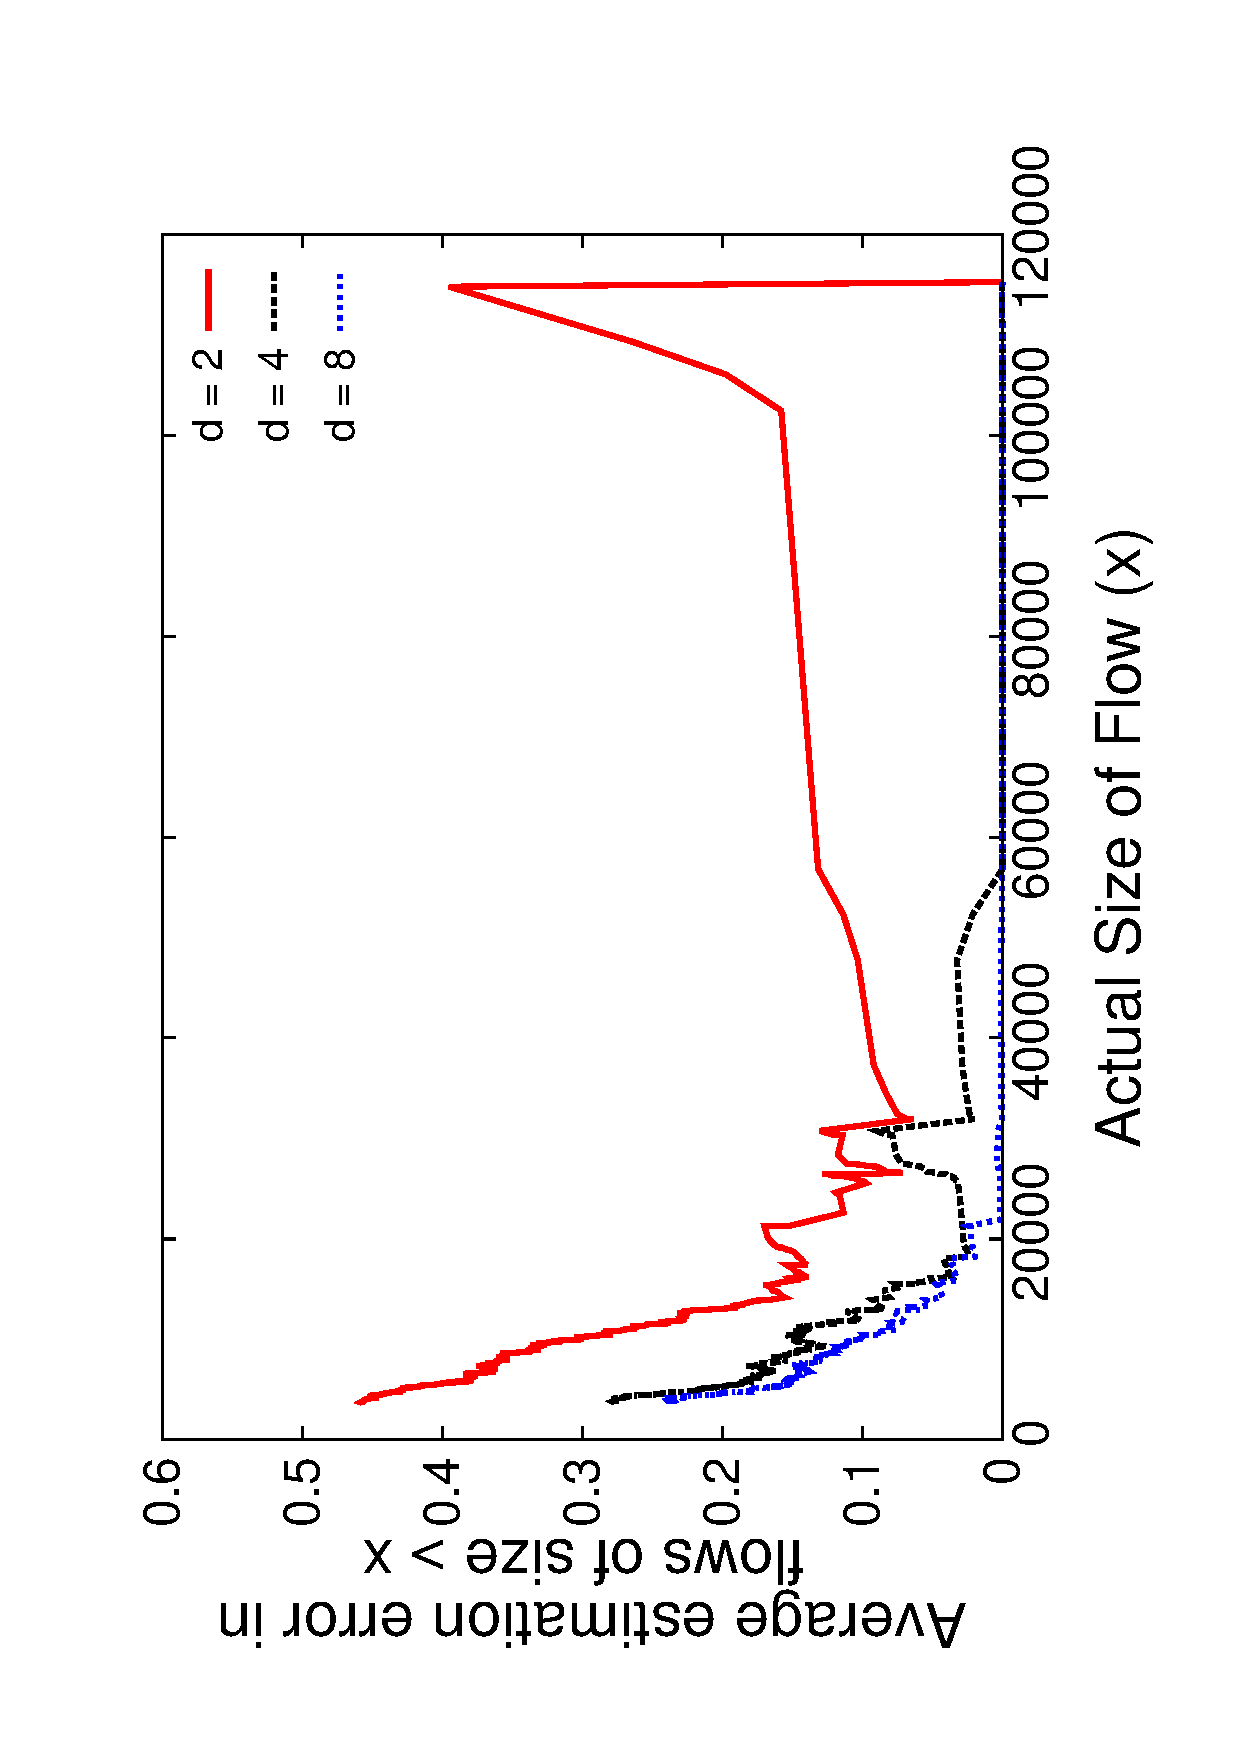
\includegraphics[max height=11cm,max width=8cm]{DsRelativeError.pdf}
\caption{Comparison of average estimation error (\%) of flows whose true counts
  are higher than the $x$-value in the graph. Error
 decreases as $d$ grows, yet, the difference is less pronounced at higher $d$}
\label{fig:estimation-error-D}
\end{figure}

%% In order to enure that the algorithm preserves the feed-forward property,
%% \TheSystem always inserts the incoming flow in stage $1$ an then computes the
%% minimum in a rolling fashion (\Sec{sec:feed-forward}). However, this could
%% induce some duplicates in the table when a flow present in a later table
%% stage is inserted afresh in the first table stage. Figure
%% \ref{fig:duplicates} shows that the fraction of the table occupied by
%% duplicates increases as the memory provisioned is increased but that this is
%% a small fraction (around $5\%$) of the total memory available for
%% heavy-hitter detection. %smaller memories, fewer %duplicates - get evicted
%% (or coalesced) for %larger flows - shows up as underestimates?


\subsection{Accuracy of \TheSystem}
\label{subsec:isolatedEvaluation}

We plot error \vs memory tradeoff curves for \TheSystem, run with $d=6$ table
stages.

\NewPara{False negatives.} \Fig{HPNegvsM} shows the false negatives as memory
increases, with curves corresponding to different numbers of reported heavy
hitters $k$. We find that error decreases with allocated memory across a range
of $k$ values, and settles to under 10\% in all cases at 80KB of memory, which
corresponds to 4500 counters.
%
For $k$=300, the error drops to about 5\% at 110KB, corresponding to 6200
($\sim20k$) counters, and for $k$=60, the error is about 2\% at the same memory
($\sim100k$).
%
%% For $k=300$, the error drops under 10\% at about 4000 counters ($\sim 13k$)
%% counters, and for $k=60$ around 2000 counters ($\sim 33k$).
%% (As memory increases beyond the range shown, false negatives continue to
%%drop.)
Recall that there are about 400,000 flows on average in any one trial,
which is two orders of magnitude higher than the number of counters used here.
We also find that the factor of $k$ required in the number of counters so as to
achieve a particular accuracy {\em reduces} as $k$ increases.

%% We also evaluate the memory-accuracy tradeoff for \TheSystem when one is
%% interested in the top-$k$ flows. Figure \ref{fig:HPNegvsM} and \Fig{HPPosvsM}
%% captures this tradeoff for different values of $k$. The trend indicates, as
%% expected, that for a given $k$ value, the accuracy improves as we provision more
%% memory. Given that the individual $20s$ traces contain around $0.5M$ flows by
%% 5-tuple on average, we are able to detect on the order of $100$ heavy flows
%% amongst the $0.5M$ with less than $10\%$ false negatives using less than $5K$
%% entries or $80 KB$ of space! This translates to needing roughly $15-20$ times
%% $k$ entries to track the top-$k$ heavy hitters to achieve a false negative rate
%% that is lower than $10\%$. At even higher memory, the false negative rate drops
%% to $5\%$. The exact factor is different across different $k$. As you increase
%% $k$, the curves start dropping faster. For example, at $k=60$, $1500$ or $25x$
%% entries are needed, while at $k=240$, less than $4500$ or $18$x entires are
%% needed.


\begin{figure}[ht]
\includegraphics[width=\columnwidth]{FalseNegsvsMsSingle.pdf} % previously [width=0.45\columnwidth]
\caption{False negatives of \TheSystem with increasing memory. Each trial trace
  contains an average of 400,000 flows, but \TheSystem achieves between 5-10\%
  false negatives for the top 60-300 heavy hitters with just 4500 flow
  counters.}
  %% Accuracy of reported Heavy hitters for Different $m$ values at $d = 6$ with
  %% $0.5M$ flows. $80KB$ translates to about 4500 key, value pairs
\label{fig:HPNegvsM}
\end{figure}


%% unsure about this figure, not turning out the way i hoped

%rephrase that it helps understand error
\NewPara{Which flows are likely to be missed?} %% We achieve a 10\% false negative
%% rate for the top 300 flows with 80KB memory, so 
It is natural to ask which flows
are more likely missed by \TheSystem. \Fig{falseNegvsK} shows how the false
negatives change as the number of desired heavy hitters $k$ is varied, for three
different total memory sizes. We find that {\em the heaviest flows are least
  likely to be missed}, \eg with false negatives in the 1-2\% range for the top
20 flows, when using 3000 counters. This trend is intuitive, since \TheSystem
prioritizes the retention of larger flows in the table
(\Sec{sec:spacesaving}). Most of the higher values of false negative errors are
at larger values of $k$, meaning that the smaller of the top $k$
flows are more likely to be missed among the reported flows.

%% While the overall false
%% negative rate that we achieve for the top-$k$ flows is around $10\%$, Figure
%% \ref{fig:falseNegvsK} indicates that if we were interested in a smaller number
%% of heavy hitters, the false negative rate would be even lower.  Given that
%% \TheSystem prioritizes heavier flows over smaller ones, as $k$ increases, the
%% false negative rate in reporting the corresponding top-$k$ heavy hitters also
%% increases.  This does indicate, though, that the majority of the errors in
%% \ref{fig:HPPosvsM} (\ref{fig:HPNegvsM}) and \ref{fig:falseNegvsD} are arising
%% from the smaller flows and the heavier flows are retained with very high
%% probability.
% typical number that might be useful for applications?
%% anything more?

\begin{figure}[h]
\includegraphics[max height=11cm,max width=8cm]{FalseNegvsKSingle.pdf}
\caption{False negatives against different numbers of reported heavy flows
  $k$. The heavier a flow is, the less likely it is missed.}
\label{fig:falseNegvsK}
%plot 600 line here too
\end{figure}

\NewPara{False positives.} \Fig{HPPosvsM} shows the false positives of
\TheSystem against varying memory sizes, exhibiting the natural trend of
decreasing error with increasing memory. In particular, we find that false
positive rates are very low, partly owing to the large number of small flows. On
all curves, the false positive rate is smaller than 0.1\%, dropping to lower
than 0.01\% at a table size of 80KB.

%\ngs{Perhaps add counter estimation errors.}

\begin{figure}[ht]
\includegraphics[width=\columnwidth]{FalsePosvsMsSingle.pdf}
\caption{\TheSystem has false positive rates of 0.01\%-0.1\% across a range of
  table sizes and reported heavy hitters.}
\label{fig:HPPosvsM}
\end{figure}

%Choose parameters for good performance of our scheme. Given a K (for top K) or threshold (for threshold HH), how do you determine
%- number of table stages? 
%- assymetry - wanna explore this at all?
%- memory size?

%(2) Memory/other overheads - get away with not keeping entire key if the goal isn't to report to the controller, but instead to act on hh directly in the dataplane

\subsection{\TheSystem\ \vs Existing Solutions}\label{subsec:comparisonRelated}

\NewPara{Comparison baselines.} We compare \TheSystem against two
schemes---representative of sampling and sketching---which are able to estimate
counts in the switch directly (\Sec{sec:related}). We use the same total memory
as earlier, and measure the top $k = 150$ flows, with the following baseline
schemes.

\noindent (1) Sample and Hold: We simulate sample and hold~\cite{estan2002new}
with a flow table that is implemented as a {\em list}.  As described in
\Sec{sec:related}, we liberally allow incoming packets to look up flow entries
anywhere in the list, and add new entries up to the total memory size. The
sampling probability is set according to the available flow table size,
following recommendations from \cite{estan2002new}.

\noindent (2) Count-min sketch augmented with a `heavy flow' cache: We simulate
the count-min sketch~\cite{cormode2005improved}, but use a flow cache to keep
flow keys and exact counts starting from the packet where a flow is {\em
  estimated to be heavy} from the sketch. We liberally allow the count-min
sketch to use the offline-estimated exact count of the $k$th heaviest
flow in the trace, as a threshold to identify heavy flows. The flow cache is
implemented as a hash table that retains only the pre-existing flow key on a
hash collision. We allocate half the available memory each to the sketch and the
flow cache.\footnote{This is similar to the memory splits used in \cite[page
    288]{estan2002new}.}

\begin{figure}[h]
\includegraphics[max height=11cm,max width=8cm]{CompFalseNeg.pdf}
\caption{Comparison of false negatives of \TheSystem to other
  baselines. \TheSystem outperforms sample and hold and count-min sketch over
  the entire memory range evaluated.}
\label{fig:FalseNegvsMSchemes}
\end{figure}

%% In order to evaluate our scheme against our two main competitors, we ran
%% \TheSystem, Count-Min Sketch with a cache and Sample and Hold on the same traces
%% with the same amount of memory (ranging from $5KB$ to $80KB$) and compared the
%% average rate of false negatives that each of the schemes produced across all the
%% traces in detecting the top $150$ flows. In the case of \TheSystem, the memory
%% provisioned is directly translated into a certain number of entries (flowid,
%% packet count pairs) in the hash table assuming that the flow-id is the 5-tuple
%% for an Ipv4 packet. For Sample and Hold, this translates into a similar number
%% of entries based on the same principle, but this is the maximum number of
%% entries that the flow memory can hold \cite{estan2002new}. For the count-min
%% sketch combined with cache, we allocate half of the memory to the sketch itself
%% and the other half to track the heavy-hitter flows in the cache, as suggested in
%% the analysis of the Multi-stage filter \cite{estan2002new}.

\NewPara{False negatives.} \Fig{FalseNegvsMSchemes} shows false negatives
against varying memory sizes, for the three schemes compared. We see that
\TheSystem outperforms sample and hold as well as the augmented count-min sketch
over the entire memory range. (All schemes have smaller errors as the memory
increases.) Notably, at 100KB memory, \TheSystem has 15\% smaller false negative
rate than sample and hold. The count-min sketch tracks the error rate of
\TheSystem more closely from above, staying within a 3-4\% error
difference. Next, we understand where the errors occur in the baseline schemes.

\NewPara{Where are the errors in the other baselines?} \Fig{relative-error}
shows the count estimation error (\%) averaged across flows whose {\em true
  count} is higher than the $x$-value in the graph, when running all the schemes
with 26KB memory.

Sample and hold can make two kinds of estimation errors. It can miss the first
set of packets from a heavy flow because of not sampling the flow early enough,
or (less likely) miss the flow entirely due to not sampling or the flow table
becoming full. \Fig{relative-error} shows that sample and hold makes
the former kind of error even for flows with very high true counts. For
example, there are relative errors of about 10\% even for flows of size more
than 80,000 packets. As \Fig{FalseNegvsMSchemes} shows, the errors becomes less
prominent as the memory size increases, since the sampling rate increases too.

The count-min sketch makes errors because of its inability to discriminate
between heavy and light flows during hash collisions in the sketch. This means
that a {\em light} flow colliding with heavy flows may occupy a flow cache
entry, preventing a heavier flow later on from entering the flow cache. For
instance in \Fig{relative-error}, even flows as large as 50,000 packets can have
estimation errors close to 20\%. However, as \Fig{FalseNegvsMSchemes} shows, the
effect of hash collisions becomes less significant as memory size increases.

On the other hand, \TheSystem's average error on flows larger than 20,000
packets---which is 0.2\% of the total packets in the interval---is negligible
(\Fig{relative-error}). \TheSystem has 100\% accuracy in estimating the count of
flows larger than 30,000 packets.

%% Fig \ref{fig:FalseNegvsMSchemes} suggests that all three schemes uniformly do
%% better at higher amounts of memory. \TheSystem outperforms both Sample and Hold
%% and the Count-min sketch based approach by over $10\%$ at smaller amounts of
%% memory, in terms of missing fewer of the heavy hitting flows. The reason for
%% this is that Sample and Hold only samples one among every so many flows,
%% depending on the sampling rate, which is decided once the flow memory size is
%% decided. Hence, it may lose some of the heavy-hitting flows altogether or may
%% sample a heavy-hitter so late in the measurement interval that its count is
%% underestimated significantly. A more detailed analysis of this effect is
%% illustrated in Figure \ref{fig:relative-error}. 

%% Count-min sketch, on the other hand, does not discriminate between packets
%% belonging to a heavy flow vs. those belonging to a small flow, in maintaining
%% information in the sketch itself. As a consequence, in the count-min sketch
%% and cache scheme, if the smaller flows collide with a few heavy hitters, the
%% heavy hitters' counters themselves are overestimated (Figure
%% \ref{fig:relative-error}) along with the smaller flows occupying the space in
%% the cache that could have gone to true heavy hitters. This effect becomes
%% less prominent as the memory is increased, as Figure
%% \ref{fig:FalseNegvsMSchemes} shows . However, this scheme does rely on
%% setting the threshold for flagging a heavy hitter accurately in the count-min
%% sketch. A lower threshold would result in a lot of flows being added to the
%% cache at the expense of true heavy hitters. A higher threshold would prevent
%% legitimate heavy hitters from even entering the cache. Given that this
%% threshold involves the knowledge of the $k_{th}$ flow's size, this is a
%% somewhat circuitous approach to identifying the $k$ heaviest
%% flows.\vls{unsure if everything is needed}

%
%- sample and hold (currently top K)
%- count min + cache (currently threshold)
%- univmon? opensketch?
%- reversible sketch?
%- XXX: need to figure out exhaustive set of comparison schemes.

\begin{figure}[h]
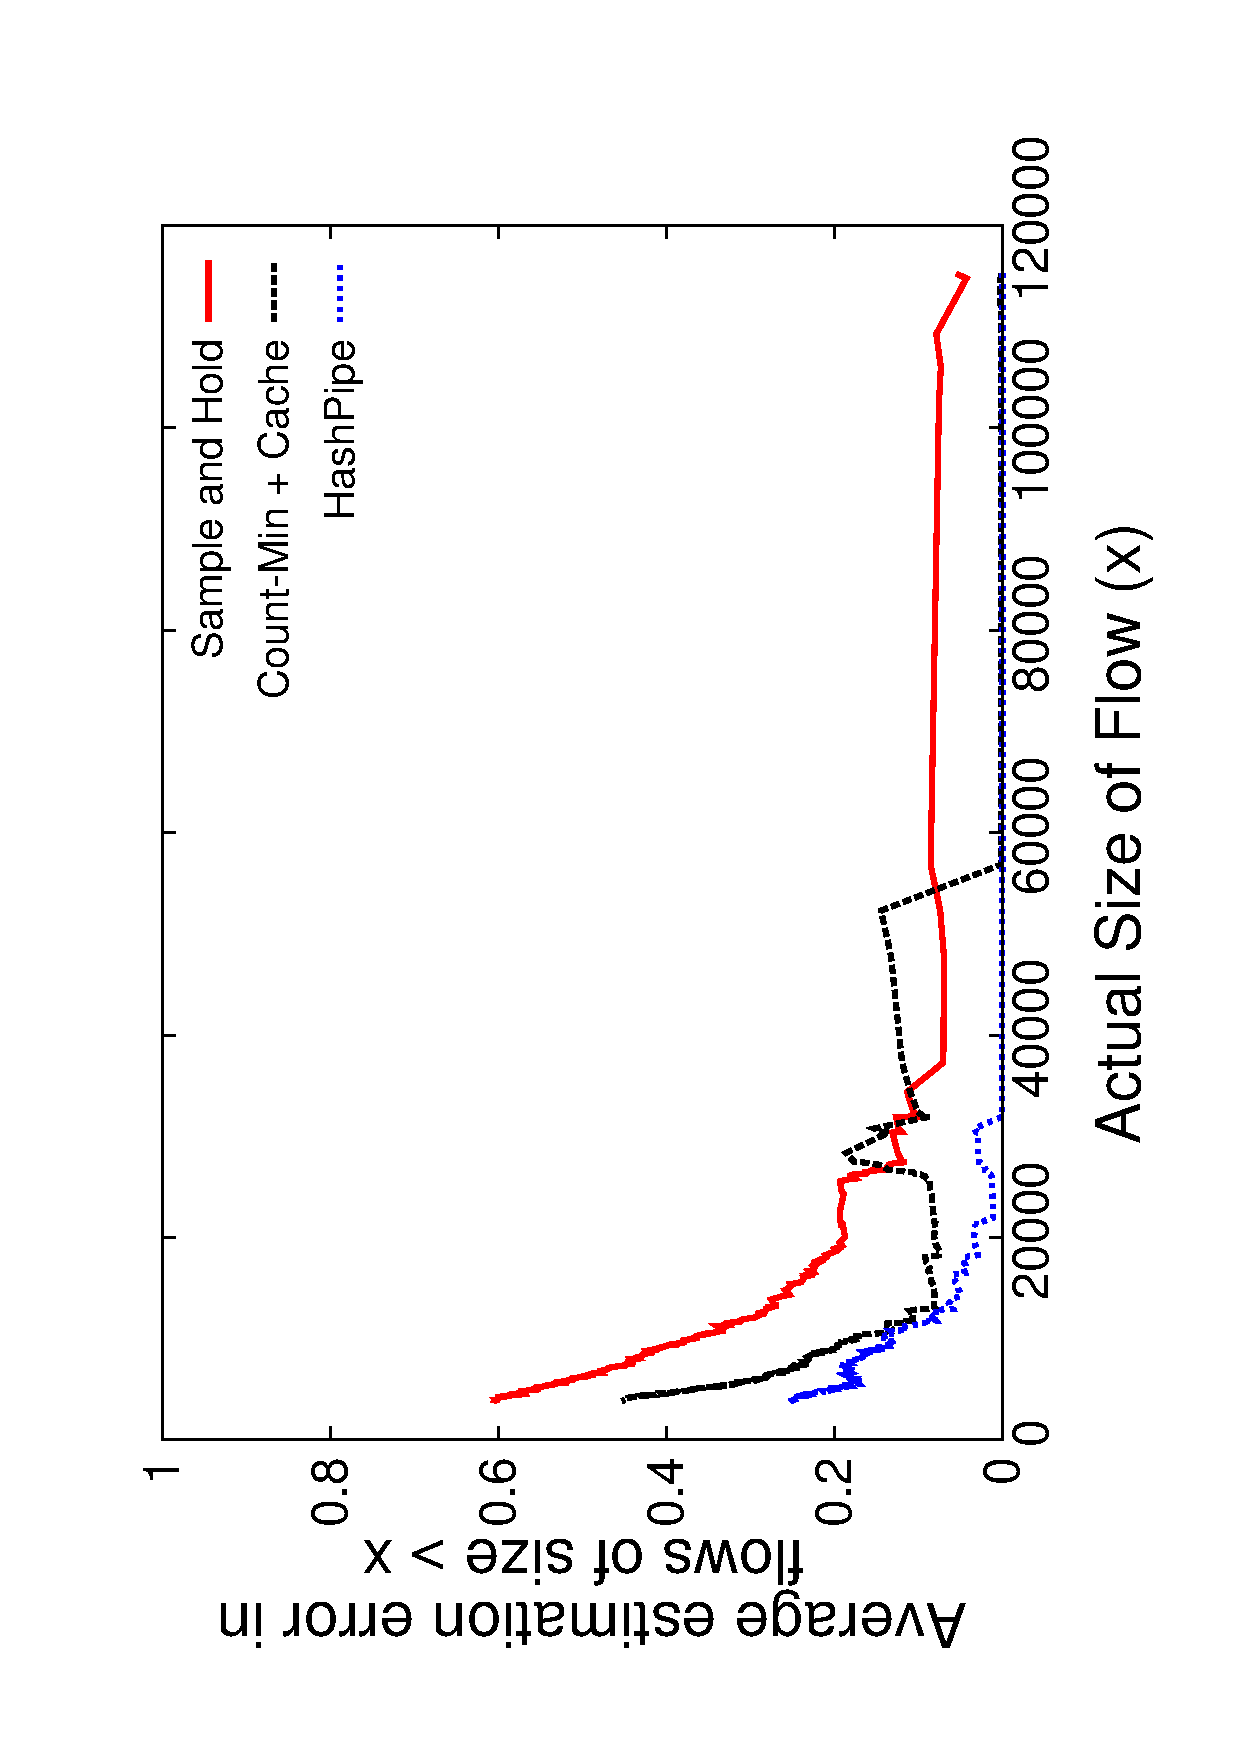
\includegraphics[max height=11cm,max width=8cm]{RelativeError.pdf}
\caption{Comparison of average estimation error (\%) of flows whose true counts
  are higher than the $x$-value in the graph. Sample and hold underestimates
  heavy flows due to sampling, and count-min sketch misses heavy flows due to
  lighter flows colliding in the flow cache. \TheSystem has no estimation errors for
  flows larger than 30,000 packets.}
  %% Comparison of average relative error in the reported sizes of flows whose
  %% actual size is larger than a given actual flow size, when detecting $150$
  %% Heavy Hitters from $0.5M$ flows on average with $26KB$ ofmemory}
\label{fig:relative-error}
\end{figure}

%% Figure \ref{fig:relative-error} analyzes the average relative error in the
%% reporting of all flows larger than a certain size $x$ across all the
%% schemes. Here, the relative error for a given flow of actual size $s_i$ and
%% reported size $r_i$ computed as $|\frac{s_i - r_i}{s_i}|$. The average
%% relative error at size $s$ is then computed as the average among the relative
%% error of all flows that are as large as and larger than $s$. For example, at
%% $x = 20K$ (which is $0.2\%$ of the total number of packets seen in this
%% interval)the average error in the reported size of all flows larger than
%% $20K$ packets is almost negligible with \TheSystem, around $10\%$ of $20K$
%% \ie $2K$ packets with the Count-Min sketch and a cache, and around $20\%$ or
%% $4K$ packets with Sample and Hold. WHle all schemes report higher flows with
%% better accuracy, \TheSystem achieves the almost $100\% $accuracy for all
%% flows of size larger than $30K$, which is faster than the other two. This
%% accounts for its ability to report the heavy hitters more accurately than
%% either of the other two.

\subsection{\TheSystem\ \vs Idealized Schemes}\label{subsec:comparisonIdeal}

We now compare \TheSystem against the idealized algorithms it is derived from
(\Sec{sec:algorithm}), namely \spacesaving~\cite{metwally2005efficient} and
\Baseline.

There are two reasons why \TheSystem may do badly relative to \spacesaving: (i)
it may evict a key whose count is much higher than the table minimum, hence
missing heavy items from the table, and (ii) it may allow too many duplicate
flow keys in the table (\Sec{sec:feed-forward}), reducing the memory available
for heavy flows, and evict heavy flows whose counts are underestimated due to
the duplicates. We showed that duplicate keys are not very prevalent in
\Sec{subsec:sensitivity}; in what follows, we understand their effects on false
negatives in the reported top $k$ flows.

\NewPara{How far is the subsampled minimum from the true table minimum?}
\Fig{mindist} shows the complementary CDF of the minimum count that was chosen
by \TheSystem, obtained by sampling the algorithm's choice of minimum at every
100th packet in a 10 million packet trace. We don't show the corresponding CCDF
for the absolute minimum in the table, which only takes on two values---0 and
1---with the minimum being 1 more than 99\% likely.\footnote{Note that this is
  different from the minimum distribution of \spacesaving, which has much larger
  values in its support.}
%
We see that the chance that \TheSystem chooses a certain minimum value decreases
rapidly as that value grows, judging from the straight-line plot on log scales
in \Fig{mindist}.
%
For example, the minimum counter has a value higher than 5 less than 5\% of the
time. There are a few larger minimum values (\eg 100), but they are rarer (less
than 0.01\% of the time). This suggests that it is unlikely that \TheSystem
experiences large errors due to the choice of a larger minimum from the table,
when a smaller counter exists.
%% srinivas: we haven't discussed why the absolute minimum distribution is so
%% skewed: possibly because we always insert keys with values 1. It seems less
%% important, though.

\begin{figure}[h]
\includegraphics[max height=11cm,max width=8cm]{minDistribution.pdf}
\caption{Complementary CDF of the minimum chosen by \TheSystem on $26KB$ of
  memory, sampled every 100th packet from a trace of 10 million packets.}
\label{fig:mindist}
%plot CM, UnivMon, Reversible
\end{figure}

%% \TheSystem aims to model the Space Saving \cite{metwally2005efficient}
%% algorithm in a hardware-amenable version by sampling a few locations to
%% estimate the minimum instead of computing the global minimum. A natural
%% question to ask is how far are we in our minimum approximation fromt the
%% global minimum. We compared the minimum picked by \TheSystem with the actual
%% minimum in the table at the same-time for the hash table update corresponding
%% to every $100_{th}$ packet in the trace. Figure \ref{fig:mindist} shows the
%% complementary cumulative distribution function for the two minima. The two
%% distributions look reasonably similar indicating that the approximated
%% minimum isn't that far off from the actual minimum and it is very rarely
%% higher than $10$. Further, the true minimum of the table is almost always $1$
%% which is also expected since we insert flows with value $1$ in the first
%% table stage. Our scheme also reports $1$ as the actual minimum majority of
%% the time.

\begin{figure}[h]
\includegraphics[max height=11cm,max width=8cm]{FriendsFalseNeg.pdf}
\caption{Comparison of false negatives of \TheSystem to idealized schemes when
  detecting $k$=150 heavy hitters. In some memory regimes, \TheSystem may
  even outperform \spacesaving, while \Baseline closely tracks \spacesaving.}
%% \caption{False Negative Rate for memory sizes when detecting $150$ heavy hitters from $0.5M$ flows across $10M$ packets}
\label{fig:FalseNegvsFriendSchemes-k150}
%plot CM, UnivMon, Reversible
\end{figure}


\begin{figure}[h]
\includegraphics[max height=11cm,max width=8cm]{FriendsFalseNeg60.pdf}
\caption{Comparison of false negatives of \TheSystem to idealized schemes when
  detecting $k$=60 heavy hitters.}
%% \caption{False Negative Rate for memory sizes when detecting $60$ heavy hitters
%%   from $0.5M$ flows across $10M$ packets}
\label{fig:FalseNegvsFriendSchemes-k60}
%plot CM, UnivMon, Reversible
\end{figure}

\NewPara{Comparison against \spacesaving and \Baseline.} We compare the false
negatives of the idealized schemes and \TheSystem against varying memory sizes
in \Fig{FalseNegvsFriendSchemes-k150} and \Fig{FalseNegvsFriendSchemes-k60},
when reporting two different number of heavy hitters, $k$=150 and $k$=60
respectively. Two features stand out from the graph for both $k$ values. First,
wherever the schemes operate with low false negative error (say less than 20\%),
the performance of the three schemes is comparable (\ie within 2-3\% of each
other). Second, there are small values of memory where \TheSystem\ {\em
  outperforms} \spacesaving.

Why is \TheSystem outperforming \spacesaving? \spacesaving only guarantees that
the $k$th heaviest item is in the table when the $k$th item is larger than the
average table count (\Sec{sec:spacesaving}). In our trace, the 60th item and
150th item contribute to roughly 6000 and 4000 packets out of 10 million
(resp.), which means that they require at least\footnote{10 million / 6000
  $\approx$ 1700; 10 million / 4000 $\approx$ 2500.} 1700 counters and 2500
counters in the table (resp.). These correspond to memory sizes of 30KB and 45KB
(resp.). At those values of memory, we see that \spacesaving starts
outperforming \TheSystem on false negatives.

We also show why \spacesaving fails to capture the heavier flows when it is
allocated a number of counters smaller than the minimum number of counters
mentioned above. Note that \TheSystem attributes every packet to its flow entry
correctly (but may miss some packets entirely), since it always starts a new
flow at counter value 1. However, \spacesaving increments {\em some counter} for
every incoming packet (\Alg{spacesaving}). In contexts where the number of
active flows is much larger than the number of available counters (\eg 400,000
flows with 1200 counters), this can lead to some flows having enormously large
(and grossly overestimated) counters. In contrast, \TheSystem keeps the counter
values small for small flows by evicting the flows (and counts) entirely from
the table.

At memory sizes smaller than the thresholds mentioned above, incrementing a
counter for each packet may result in {\em several small flows} catching up to a
heavy flow, leading to significant false positives, and higher likelihood of
evicting truly heavy flows from the table. We show this effect on \spacesaving
in \Fig{SSkeysperbucket} for $k$=150 and $m$=1200 counters ($m$=2500 needed).
The distribution of the number of keys contributing to a false positive flow
counter in the table is clearly shifted to the right relative to the
corresponding distribution for a true positive flow counter.
%
%% A similar and
%% natural characterization of the distributions holds for the estimation errors
%% from the different categories of flow keys, shown in \Fig{SSdevperbucket}.

%% To quantify how we do compared to \spacesaving, we compared the performance of
%% \TheSystem against the intermediate \Baseline as well as \spacesaving in terms
%% of the false negative rate in the reporting of $150$ heavy hitters with
%% different amounts of memory. As reported in Figure
%% \ref{fig:FalseNegvsFriendSchemes}, \Baseline is almost identical to \spacesaving
%% in its performance. This is not surprising since Figure \ref{fig:mindist} shows
%% that sampling the minimum doesn't result in such a different distribution from
%% the actual minimum. However, \TheSystem has significantly lower false negative
%% rates (by almost $15\%$) than either of them at almost all memory sizes. This is
%% attributed to the fact that \TheSystem inserts a new flow with value $1$ in the
%% first table while \spacesaving and \Baseline both replace it with the current
%% minimum value incremented by $1$.

\begin{figure}[h]
\includegraphics[max height=11cm,max width=8cm]{SSKeysPerBucketDist.pdf}
\caption{CDF of the number of distinct flows contributing to a counter in
  \spacesaving's table, when identifying $k$=150 heavy flows with $m$=1200
  counters. We show three distributions according to the flow's label after the
  experiment.}
%% \caption{Chances of a given bucket having a certain number of keys contributing
%%   to it when running \spacesaving to identify $150$ heavy hitters with $1200$
%%   counters. Legend represents category that the flow found in a bucket at the
%%   end of the interval belongs to.}
\label{fig:SSkeysperbucket}
\end{figure}

%% When the number of flows and packets in a network are high (around two orders
%% of magnitude more than the number of entries in the table), the fact that
%% every packet causes at least one counter to increment by $1$
%% \cite{metwally2005efficient} without any evictions results in a large average
%% counter value.  This large average counter could be even larger than some of
%% the heavy hitter flows resulting in certain mice flows being incorrectly
%% reported while other legitimate hevay hitters are missed. To analyze this, we
%% observed the number of keys that contributed to the count in every bucket at
%% the end of the measurement interval in Space-Saving when run with $1200$
%% counters. In addition, we analyzed what the reported size of the flow in the
%% bucket was and how it compared to the actual size of the flow (relative error
%% of that flow). We then classified the flows based on whether they were True
%% Positives, False Positives or neither in the context of the top $150$ flows.

%% \begin{figure}[h]
%% \includegraphics[max height=11cm,max width=8cm]{SSDeviationPerBucketDist.pdf}
%% \caption{CDF of the count estimation error (\%) of different flows in
%%   \spacesaving's table, when identifying $k$=150 heavy flows with $m$=1200
%%   counters. We show three distributions according to the flow's label after the
%%   experiment.}
%% \label{fig:SSdevperbucket}
%% \end{figure}

%% Figure \ref{fig:SSkeysperbucket} shows that the number of keys contributing to a
%% particular bucket is over $2000$ in more than half the buckets. If each of those
%% keys contributed even two packets, that would be over the actual true count of
%% the average $150^{th}$ ranked flow. Thus even a few such buckets would start
%% competing heavily against the true heavy hitters, as illustrated in the false
%% positive line of the plot. Similarly, according to Figure
%% \ref{fig:SSdevperbucket}, the relative error with those flows in the table that
%% are not true positives is so high that it indicates the possibility that if
%% these were medium-sized in the first place, they could, once again, easily
%% replace the true-positives.

\NewPara{Impact of duplicate keys in the table.} Finally, we investigate how
duplicate keys and consequent underestimation of flow counts in the table may
affect the errors of \TheSystem. In \Fig{reportingMoreThanK-falseneg}, we show
the benefits of reporting {\em more than $k$ counters} on false negatives, when
the top $k$=300 flows are requested with a memory size of $m$=2400 counters.
While the false negative rates of \spacesaving and \Baseline improve
significantly with overreporting, the errors for \TheSystem remains flat
throughout the interval, dropping only around 1800 reported flows. We infer that
most heavy flows are retained somewhere in the table for \spacesaving and
\Baseline, while \TheSystem underestimates keys sufficiently often that they are
completely evicted---to the point where overreporting does not lower the false
negative errors. \Fig{reportingMoreThanK-falsepos} shows that overreporting
flows only increases the false positive errors slightly for all schemes, with
values staying between 0.1-0.5\% throughout.

\begin{figure}[h]
\includegraphics[max height=11cm,max width=8cm]{FriendsFalseNegWithRep.pdf}
\caption{Benefits of overreporting flows from the table on false negative errors
  with $k$=300 heavy flows and $m$=2400 counters. While \spacesaving and
  \Baseline improve significantly when reporting even as many as $2k$ flows,
  \TheSystem does not, because of evictions due to duplicate entries.}
%% \caption{
%%   Comparison of false negatives of HashPipe to \spacesaving and Hash
%%   Parallel when reporting more than $k$ candidate flows. \spacesaving and
%%   HashParallel significantly outperform HashPipe even with $2k$ reported flows}
\label{fig:reportingMoreThanK-falseneg}
\end{figure}

\begin{figure}[h]
\includegraphics[max height=11cm,max width=8cm]{FriendsFalsePosWithRep.pdf}
\caption{Impact of overreporting flows from the table on false positive errors
  with $k$=300 heavy flows and $m$=2400 flows. %%The errors stay within a small
  %%range.}
  }
\label{fig:reportingMoreThanK-falsepos}
\end{figure}

%%
%- scatter plots to show where errors arise in our scheme. Sources of error include effect of hash collisions and packet interleaving. Possibly talk about prevalence of duplicates in sequential probing as a source of error. (generate graph here)
%- impact of (i) subsampling the table (as opposed to looking at the entire table), assuming you see all $D$ probes at once (ii) partial knowledge/sequential lookup instead of seeing all $D$ locations at once.
%(the two categorizations above may lead to the same!)
%%

%%

%zoomed in only top 1000 flows
%Focusing on only the top 1000 flows
%\includegraphics[max height=11cm,max width=8cm]{image031}
%\includegraphics[max height=11cm,max width=8cm]{image033}



\section{Related Work}
\label{sec:other-related}

\NewPara{Applications that use heavy hitters.} Several applications
use information about heavy flows to do better traffic
management or monitoring. DevoFlow~\cite{devoflow} and
Planck~\cite{planck} propose exposing heavy flows with low overhead as ways to
provide better visibility and reduce congestion in the
network. UnivMon~\cite{univmon} uses a top-$k$ detection sketch internally as a
subroutine in its ``universal'' sketch, to determine more general statistics
about the network traffic. There is even a P4 tutorial application on switch
programming, that performs heavy hitter detection using a count-min-sketch-like
algorithm~\cite{p4-sigcomm-tutorial-hh-example}.

\NewPara{Measuring per-flow counters.} Several prior works like
FlowRadar~\cite{li2016flowradar}, CounterBraids~\cite{counterbraids}, and
others, \eg~\cite{li-randomized-counter-sharing} have proposed schemes to
measure accurate per-flow traffic counters. Along similar lines, hashing schemes
like cuckoo hashing~\cite{cuckoo-hashing} and d-left
hashing~\cite{vocking2003asymmetry} can keep per-flow state memory-efficiently,
while providing fast lookups on the state. Our goal is not to measure or keep
all flows; just the heavy ones. We show (\Sec{sec:evaluation}) that \TheSystem
uses 2-3 orders of magnitude smaller memory relative to having per-flow state
for all active flows, while identifying more than 95\% of the heavy flows.

\NewPara{Other heavy-hitter detection approaches.} The multi-resolution tiling
technique in ProgME~\cite{progme}, and the hierarchical heavy-hitter algorithm
of Jose \etal~\cite{jose2011online} solve a similar problem as
ours. They estimate heavy hitters in traffic {\em online}, by iteratively
refreshing the set of packet counters on a switch and ``zooming in'' to the
portions of traffic which are more likely to contain heavy flows. However, these
algorithms require the involvement of the control plane to run their
flow-space-partitioning algorithms, while \TheSystem works completely within the
switch pipeline. Further, both prior approaches require temporal stability of
the heavy-hitter flows to detect them over multiple intervals; \TheSystem
determines heavy hitters using the counters updated within the same interval.

%%- https://www.cise.ufl.edu/~sgchen/paper/sigmetrics2015.pdf
%% frameworks/apps: opensketch
%% packet mirroring: everflow, netsight
%% other monitoring: latency/loss measurement. LDA, reference latency
%%   interpolation, etc.
%% other apps: flow size distribution? billing?
%% other hash-based schemes? see survey of kirsch, varghese and mitzenmacher

%% "Our approach efficiently allocates the available space to the heavy hitters by either evicting a large number of the small flows on a packet-by-packet basis or restricting them to a small subset of the entire table space. This proves to be a crucial advantage in estimating the heavy hitters more accurately when compared to other existing schemes"


%% Group Testing - larger number of counters - many more tables as k increased - too much space to less important items - key recoverable
%% Space-Saving is the most space-efficient way of maintaining information

%% Really bad space-complexity they devote too much space to less imp items
%% Or major background processing to be able to scan or clean or evict items once in a while - amortized O(1)
%% We want something that is deterministically O(1)

%% Candidates:
%% - count-min: no keys here; only do top-k (no threshold)
%% - count-min + reversible sketch -- [XXX: why is this inaccurate?]. decoding overhead
%% - sample and hold: [XXX: inaccurate for the same amount of memory... but why?]
%% --> can we use the bounds from these papers?
%% - univmon?
%% - flowradar?
%% - other streaming heavy hitters algorithms (e.g., space savings) --> can't do on general purpose switch hardware
%% - discuss the fact that space saving achieves the lower bound of O(k)

%%\input{discussion}
\section{Conclusion}\label{sec:conclusion}

%In the paper, we studied the constraints switch architectures apply on
%algorithm implementations in order to maintain high packet processing.
%Focusing on heavy hitter detection, we design an algorithm that follows these
%restrictions while still achieving high accuracy.

In this paper, we proposed an algorithm to detect heavy traffic flows within the
constraints of emerging programmable switches, and making this information
available within the switch itself, as packets are processed. Our solution,
\TheSystem, uses a pipeline of hash tables to track heavy flows preferentially,
by evicting lighter flows from switch memory over time. We prototype \TheSystem
with P4, walking through the switch programming features used to implement our
algorithm. Through simulations on a real traffic trace, we showed that
\TheSystem achieves high accuracy in finding heavy flows within the memory
constraints of switches today.%%  while outperforming existing heavy-hitter
%% detection schemes that use sampling and sketching.
%% In this paper, we discussed the constraints imposed by switching architectures on
%% algorithmic implemenations due to the need for high speed packet processing. In
%% particular, we propose an algorithm for heavy hitter detection called \TheSystem
%% that respects these restrictions while still achieving high accuracy. \TheSystem
%% uses a pipeline of hash tables along with a local minimum computation at each
%% pipeline stage to preferentially track the heavier flows. We also prototype the
%% algorithm in P4. Through our simulations, we show that \TheSystem achieves lower
%% error rates than existing sampling and sketching based approaches %like Sample
%%                                 %and Hold and Count-Min Sketch 
%% at comparable amounts of memory.
%% We are further studying \TheSystem through synthetic workloads, additional
%% optimizations to the algorithm, and theoretical analyses.

%univmon, dataplane
% assymmetric memory split
%synthetic workloads
%compiling to a target
%extensive analysis

\label{lastpage}

%\begin{appendices}
%%%\section{Analysis}

\newtheorem{lemma}{Lemma}
\newtheorem{theorem}{Theorem}

%Discuss heaps/ideal space-saving to be used as reference

%\subsection{All probes available at once}
%\subsubsection{Aggregate Model}
%\subsubsection{Cash Register Model}
%\subsection{Accomodating HW constraints}
%\subsubsection{Aggregate Model}
%\subsubsection{Cash Register Model}

%% \subsection{Algorithm}

%% Let table $T$ represent a table of items and corresponding counts. The table has
%% a fixed size $M$, with some table locations possibly empty. A nonempty table
%% location contains an element $e$ and a corresponding counter $c$, denoted as
%% $(e,c)$. Each incoming item $p$, \eg a packet, is independently hashed to $d$
%% locations in table $T$, denoted by the set $H_p$. Consider the following
%% algorithm.\\

%% \noindent For each item $p$\\
%% hash $p$ to table locations $H_p = \{l_1, l_2, \ldots, l_d\}$ with $l_i = (e_i, c_i)$\\
%% if $\exists i: p = e_i$ then $c_i \leftarrow c_i + 1$\\
%% else if $\exists j: l_j$ empty then $e_j \leftarrow p; c_j \leftarrow 1$\\
%% else let $k \leftarrow \mathrm{arg min}_{k \in \{1,\ldots,d\}} \ c_k; e_k \leftarrow p; c_k \leftarrow c_k + 1$\\

\section{Overestimation Errors}
\label{sec:analysis}

We show that \Baseline (\Alg{Baseline}) does not overestimate keys by too much
when it samples the minimum of $d$ slots in the table, instead of the entire
table.

First, note how it is possible to overestimate the frequency of an item
$e_i$. Suppose on its insertion $e_i$ replaces another item $e_j$ in $T$, where
$e_j$ is the element with the minimum counter among locations that $e_i$ hashed
to. Independent of the true count of item $e_i$ so far (say, zero), its counter
is set to $c_j + 1$.

\begin{lemma}
For any item $e_i$ in $T$ (with table count $c_i$), let $min_i$ denote the
minimum counter value among the locations that $e_i$ hashes to. That is, $min_i
= \mathrm{min}_{(e_j,c_j) \in H_i} \ c_j$. Let $f_i$ denote the true count of
$e_i$. Then, $c_i \leq f_i + min_i$.
\end{lemma}

\begin{proof}
Consider an item $e_i$ in $T$, and the last time that $e_i$ was inserted into
the table. Suppose the minimum counter value among the $d$ locations that $e_i$
hashed to at the time of its insertion be $m_i$. Also suppose that $e_i$
occurred $n_i$ times after its last insertion in the table. Clearly, $c_i = m_i
+ n_i$.

The minimum counter among the $d$ locations in $H_i$ is monotonically
increasing, since the algorithm never decrements any counters. Hence, $m_i \leq
min_i$. Further, since $n_i$ can be at most $f_i$, the lemma follows.
\end{proof}

\begin{lemma}
For a fixed $\delta \leq 1$, with probability at least $1 - \delta^d$, we have
$min_i < N/\delta M$.
\end{lemma}

\begin{proof}

We wish to bound the value of $min_i$ from above. Suppose there are $N$ packet
arrivals overall. Since every item arrival contributes to an increment in $T$,
the expected value of a counter in $T$ is $N/M.$ Hence, the minimum counter in
$T$ can be at most the expected value, \ie $N/M.$ However, the minimum in $H_i$ for an
item $i$ can in general be quite far from the minimum of $T$.

It can be shown that the minimum in $H_i$ is still unlikely to be much larger
than the bound on the minimum above. The expected value of the counters in $T$
is $N/M$, so by the Markov inequality the probability that a randomly chosen
item has a counter value higher than $N/\delta M$ is no more than
$\delta$. Then, the chance that the minimum of $d$ randomly chosen elements is
higher than $N/\delta M$ is at most $\delta^d$. Hence with probability at least
$1 - \delta^d$, we have $min_i \leq N/\delta M$.

\end{proof}

%% \subsection{Underestimation errors}

%% It is possible to underestimate the counts of items within the table, or miss
%% heavy items entirely, through this algorithm. To see why, consider a simple
%% example with $d=2$. Suppose item $e_i$ hashes to two locations $l_1$ and $l_2$,
%% occupying location $l_1$ with counter $c_1$. Further, suppose that $l_2$ is
%% occupied with another item with count $c_2^{evict} < c_1$. Now an item $e_j$ may
%% enter $T$, hashing to locations $l_1$ and $l_3$, where the corresponding counter
%% value $c_3 > c_1$. Then $e_j$ will evict $e_i$. However, if $e_i$ returns, the
%% counter at $l_2$ may still have a smaller value than the original count of
%% $e_i$, \ie $c_2^{reappear} < c_1$. Then the current estimate of item $i$ would
%% be smaller than its true count by $c_1 - c_2^{reappear}$. If $c_2^{reappear}$ is
%% small enough that $e_i$ is evicted later, and $e_i$ never reappears, the
%% algorithm may also miss $e_i$ entirely from the table.

%% \noindent {\bf Speculative proof ideas.} We want to show that the impact of
%% underestimations on counter values in $T$ is not significant. Suppose we call
%% $c_1 - c_2^{reappear}$ the {\em underestimation error.} One specific idea is to
%% show that the {\em average-case} underestimation error for items in $T$ is
%% small, as follows.

%% For the underestimation error to be positive-valued, it is necessary that there
%% is an item $e_j$ hashing to $d$ locations---including the location that $e_i$
%% resides in---with $d-1$ counter values each larger than $c_1$. When $c_1$ is
%% large, the likelihood of $d-1$ randomly chosen counters each being larger than
%% $c_1$ must be small. On the other hand, if $c_1$ is small, the underestimation
%% error is itself small because the gap between $c_1$ and $c_2^{reappear}$ is
%% likely to be small. Putting these two cases together, we hope to show that the
%% average-case underestimation error for any item must be small.

% want to say that underestimatin is no more than constant times N/M, how many times it gets evicted and everytime it gets evicted what the underestimate amount
% 

%\end{appendices}

%\end{sloppypar}

%\vspace{-0.1in}
%\section*{Acknowledgments}
% Comments for people we need to acknowledge in the final version.
\begin{acks}
  We thank the anonymous SOSR reviewers, Anirudh Sivaraman, and Bharath
  Balasubramanian for their feedback.  This
  work was supported partly by NSF grant CCF-1535948, DARPA grant
  HR0011-15-2-0047 and gifts from
  Intel and Huawei. We also thank the industrial members of the MIT Center for
  Wireless Networks and Mobile Computing (Wireless@MIT) for their support.

\end{acks}

%\pagebreak

\clearpage
%\setlength{\bibsep}{0pt}
\setlength{\parskip}{-1pt}
\setlength{\itemsep}{-1pt}
 \footnotesize % SPACE

\bibliographystyle{abbrv}
\begin{small}
\bibliography{paper}
\end{small}
%\bibliographystyle{abbrvnat_noaddr} % SPACE
%\theendnotes % ENDNOTES

%}
{% onlyAbstract
}

\ifappendix
\clearpage
\appendix
\input{appendix}
\fi
\end{document}

%%%%%%%%%%%%%%%%%%%%  END OF DOCUMENT  %%%%%%%%%%%%%%%%%%%%
